% !Mode:: "TeX:UTF-8"
%!TEX program  = xelatex

%\documentclass[no-math]{cumcmthesis}
\documentclass[no-math,withoutpreface,bwprint]{cumcmthesis} %去掉封面与编号页

\usepackage[T1]{fontenc}
\usepackage{newtxtext, newtxmath}
\usepackage{float}
\usepackage{tikz}
\usetikzlibrary{shapes.geometric, arrows}

\tikzstyle{startstop} = [rectangle, rounded corners, minimum width = 2cm, minimum height=1cm,text centered, draw = black]
\tikzstyle{io} = [trapezium, trapezium left angle=70, trapezium right angle=110, minimum width=2cm, minimum height=1cm, text centered, draw=black]
\tikzstyle{process} = [rectangle, minimum width=3cm, minimum height=1cm, text centered, draw=black]
\tikzstyle{decision} = [diamond, aspect = 3, text centered, draw=black]
% 箭头形式
\tikzstyle{arrow} = [->,>=stealth]

\newcounter{rowno}
\numberwithin{equation}{section}
\numberwithin{figure}{section}
\numberwithin{table}{section}
\renewcommand{\thefigure}{\arabic{section}-\arabic{figure}}
\renewcommand{\thetable}{\arabic{section}-\arabic{table}}
\renewcommand{\theequation}{\arabic{section}-\arabic{equation}}

\usepackage{url}
\title{基于模拟退火算法的RGV动态调度研究 }
\tihao{\quad B}
\baominghao{\quad 201819060022}
\schoolname{哈尔滨工业大学(深圳)}
\membera{\quad 罗彧宁}
\memberb{\quad 杨敬轩}
\memberc{\quad 蔡紫宴}
\supervisor{\quad 无}
\yearinput{2018}
\monthinput{09}
\dayinput{16}

\begin{document}

 \maketitle
 \begin{abstract}
本文针对不同加工情况下智能RGV动态调动问题,构建了基于最短路径贪心算法、及改良的模拟退火算法的动态调度模型,运用了 MATLAB编程求解以及FlexSim模拟加工过程,给出针对一道工序,两道工序以及考虑故障情况时一道工序和两道工序四种RGV动态调度方案,以及两道工序下分配8台CNC装配不同加工刀具排布的方案,并给出以绝对理想情况为比较依据的系统的作业效率。

本文的突出特点是使用了RGV每次移动均考虑当前最优解的贪心算法,以及避免暂时困于局部最优解的模拟退火算法,寻找局部乃至全局最优解,并且遍历CNC的所有工序分配方案以优化最优解。 

针对不考虑故障时一道工序的情况,我们采用贪心算法的思想建立{\bfseries\song 模型I}—基于贪心算法求解最优动态调度方案模型,由于CNC加工时长远大于RGV移动以及上下料时间,此时得到的局部最优解即为全局最优解,经 3 组数据检验,系统的作业效率约为 92\%,已经达到了全局最优。

针对不考虑故障时两道工序的情况,我们基于贪心算法的思想建立{\bfseries\song 模型II}—基于贪心算法求解最优动态调度方案模型,遍历加工不同分组下不同工序CNC数量以及排布的254种情况,以优化局部最优解,得到对于CNC分类以及排布的最优解,发现不同数据组下存在并行最优解以及唯一最优解。此模型下系统的作业效率约为89\%。

针对考虑故障时一道工序的情况,首先创新性地定义了考虑故障时一道工序情况下 CNC 剩余工作时间矩阵,基于模拟退火算法建立了{\bfseries\song 模型III}—基于模拟退火算法求解最优故障动态调度方案模型:一道工序。当给CNC进行上料操作时,对CNC进行一次故障检测,若有故障,则通过均匀分布生成此次故障发生的具体时间以及人工需要维护的时间,然后根据贪心算法重新选择最优路径,寻找局部最优解,并以一定的概率寻找倒数第二短的可行路径,多次运行以求得全局最优解。此时系统的作业效率约为 89\%。

针对考虑故障时两道工序的情况,定义了考虑故障时两道工序情况下 CNC 剩余工作时间矩阵,基于模拟退火算法的思想建立了{\bfseries\song 模型IV}—基于模拟退火算法求解最优故障动态调度方案模型:两道工序。在模型III中已经寻找到针对三组不同数据的最佳工序分配方案,模型IV延续此方案并对模型III的思想进行推广。经数据检验,模型较好的实现了有故障发生时两道工序情况下RGV 的动态调度,系统的作业效率约为 85\%。

本文为进一步增加可视化程度,保证逻辑与运算结构的清晰性,运用FlexSim进行仿真模拟,绘制模型的算法流程图和RGV动态调动示意图。本文逻辑清晰,创新性地定义了考虑故障时CNC的剩余工作时间矩阵,统一了模型I和模型III、模型II和模型IV的表达式,合理进行误差评估以及灵敏度分析,拟合实际情况并加以推广。 

\keywords{模拟退火算法;贪心算法;最短路径;RGV;动态调度;作业效率}
\end{abstract}

\vspace{-1.3cm}%使第一节标题位于最上方

\section{问题重述}

\subsection{背景知识}

\subsubsection{引言部分}

智能加工系统是一种由智能机器和人类专家共同组成的人机一体化智能系统,它在制造过程中能以一种高度柔性与集成度高的方式,借助计算机模拟人类专家的智能活动进行分析、推理、判断、构思和决策等,从而取代或者延伸制造环境中人的部分脑力劳动。智能加工系统已经成为现代化生产的大趋势。

\subsubsection{动态调度}

动态调度通常是指在调度环境和任务存在不可预测扰动情况下所进行的调度。与静态调度相比,动态调度能够针对生产现场的实际情况产生更具可操作性的决策方案。实际生产中的大量问题是随机发生的。如在机械制造业中, 由于工件随机到达, 加工机器出现故障等随机事件, 使得预调度不能正常执行, 这就需要安排重调度。

\subsubsection{研究意义}

大部分离散制造企业属于多品种小批量的生产模式,特点为产品品种多、数量少、生产重复性小、工艺过程经常变更等。因此需要一个先进适用的管理系统,对于下达的生产任务进行一定程度上的智能优化调度,最大程度地减少生产过程中的非增值时间,实现加工生产的高效率、高柔性和高可靠性。

\subsection{相关数据}

1. 题目提取:见表\ref{data}
\setcounter{rowno}{0}
\begin{center}
\begin{table}[H]
\centering
\setlength{\abovecaptionskip}{0pt}
\setlength{\belowcaptionskip}{0pt}
\caption{智能加工系统数据}
\label{data}
\begin{tabular}{>{\stepcounter{rowno}\therowno}ccc}
 \toprule[1.5pt]
\multicolumn{1}{c}{序号}& \makebox[0.4\textwidth][c]{名称}	&  \makebox[0.1\textwidth][c]{数量} \\ \midrule
& 计算机数控机床(CNC) & 8台 \\ 
 &轨道式自动引导车(RGV)& 1辆 \\ 
 &RGV直线轨道 &1条 \\ 
 &上料传送带 & 1条 \\ 
&下料传送带	    & 1条  \\
 \bottomrule[1.5pt]
\end{tabular}
\end{table}
\end{center}

2. 智能加工系统作业参数的3组数据表(见原题表1)

\subsection{具体任务}

{\bfseries\song1.任务一}

分别根据以下三种情况:一道工序的物料加工作业,两道工序的物料加工作业,考虑CNC以1\%的概率发生故障,给出RGV动态调度模型和相应的求解算法。

{\bfseries\song2.任务二}

利用题目中表1给出的系统作业参数的3组数据,代入上述算法,给出RGV的调度策略和系统的作业效率。

\section{问题的分析}

\subsection{研究现状综述}

国内外学者对RGV系统的优化做了一些研究,主要集中于RGV的派遣规则、路径选择及环轨多RGV系统的死锁避免等方面的仿真研究,但对RGV的单线往复动态调度问题的研究却几乎没有。

Dotoli和Fanti应用着色赋时Petri网提出了RGV与巷道堆垛机的物料搬运系统的模块化建模框架\upcite{bib:one}。Chen等研究了FMS中的RGV调度和控制系统\upcite{bib:two}。吴长庆等提出了基于双层着色赋时Petri网的RGVs系统的动态模型,并采用最短路径的调度策略\upcite{bib:three}。陈华等针对自动化立体仓库出库过程中的直线往复两穿梭车(RGV)系统可能存在的RGV相互碰撞问题,提出了RGV冲突避免的约束条件\upcite{bib:four}。杨少华等用排队论对环轨多车情况下的RGV数量和能力进行了分析\upcite{bib:five}。吴焱明等使用仿真的方法研究了环轨RGV系统的动态调度问题,分析对比了两种RGV调度方法\upcite{bib:six}。

总而言之,现有的文献或多或少都有其不足之处,需要加以完善。

\subsection{对问题的总体分析和解题思路}

本题需要研究的问题是智能RGV的动态调度方案的设计,包含加工一道工序的物料,加工两道工序的物料和考虑CNC在加工过程中出现故障时加工一道工序和加工两道工序四种情况,并据此对题目中表1的三组数据进行模型和算法的检验。针对此问题,我们分为四个小问题来进行研究。第一,利用MATLAB编程,对CNC加工一道工序物料的情况进行RGV的动态调度方案设计,并求解;第二,利用MATLAB编程,考虑工序分配,对CNC加工两道工序物料的情况进行RGV的动态调度方案设计,并求解;第三,针对CNC在加工过程中以1\%的概率发生故障时加工一道工序物料的情况,在10到20分钟的误工时间后加入工作队列,重新设计算法,并求解;第四,针对CNC在加工过程中出现故障时加工两道工序物料的情况,改进前面的模型,并求解。

根据本文的研究思路,做出整体的思路流程图,如图\ref{figtotal}所示。

%\begin{figure}[!h]
%	\centering
%	\includegraphics[width=0.9\textwidth]{total.pdf}
%	\caption{任务标价的统计}
%     \label{figtotal}
%\end{figure}

\begin{figure}[!h]
\centering
\begin{tikzpicture}[node distance=1cm]
%定义流程图具体形状
\node[startstop](start){开始};
\node[process, below of = start, yshift = -1cm](pro1){\quad 设计一道工序的动态调度算法并求解\,\,\,\,\,};
\node[process, below of = pro1, yshift = -1cm](pro2){\quad 设计两道工序的动态调度算法并求解\,\,\,\,\,};
\node[process, below of = pro2, yshift = -1cm](pro3){\quad 设计考虑故障时一道工序的动态调度算法并求解\,\,\,\,\, };
\node[process, below of = pro3, yshift = -1cm](pro4){\quad 设计考虑故障时两道工序的动态调度算法并求解\,\,\,\,\, };
\node[startstop, below of = pro4, yshift = -1cm](stop){结束};
%连接具体形状
\draw [arrow] (start) -- (pro1);
\draw [arrow] (pro1) -- (pro2);
\draw [arrow] (pro2) -- (pro3);
\draw [arrow] (pro3) -- (pro4);
\draw [arrow] (pro4) -- (stop);
\end{tikzpicture}
\vspace{0.4cm}
\caption{整体思路流程图}
\label{figtotal}
\end{figure}

\subsection{对具体任务的分析和对策}

{\bfseries\song1.对任务一的分析和对策}

任务1要求对一般问题进行研究,给出智能RGV的动态调度方案的设计,包含加工一道工序的物料,加工两道工序的物料和考虑CNC在加工过程中出现故障时一道工序和两道工序四种情况。针对此问题,首先,利用MATLAB编程,基于贪心算法进行加工一道工序的物料时RGV的动态调度方案设计;其次,假设三种不同的工序分配方案:第一道工序与第二道工序各自4台CNC,执行第一道工序的CNC数目大于执行第二道工序的CNC数目,执行第一道工序的CNC数目小于执行第二道工序的CNC数目,将一道工序的算法推广至两道工序,同样是基于贪心算法;最后,考虑CNC在加工过程中发生故障的情况,按照1\%的概率随机设置CNC停止工作,在10到20分钟的误工时间后加入工作队列,误工时间由区间[10, 20]内的均匀分布产生。根据模拟退火算法的思想建立模型,跳出局部最优解,以寻找全局最优解。

{\bfseries\song2.对任务二的分析和对策}

任务2要求利用3组数据分别检验算法的有效性,给出RGV的调度策略和系统的作业效率,并将具体的结果分别填入附件2的EXCEL表中。在任务1中已经得到在有无故障两种情况下三种不同工序分配方案的RGV动态调度模型,将题目中表格1的数据分别带入相应模型的算法中,使用MATLAB求解,可得最终结果。

\section{模型的假设}
\begin{enumerate}[label=\arabic*.]
\item 假设CNC在不工作时不会发生故障 
\item 假设RGV、传送带等设备在工作中不会发生故障
\item 假设物料供给及时且充足,不会出现断料的情况
\item 假设RGV内部程序的运行时间可以忽略不计
\item 假设RGV在加工两道工序的物料时,第一道工序完成后不清洗物料
\item 假设题目所给数据真实正确

\end{enumerate}

\section{名词解释与符号说明}

\subsection{名词解释}

{\bfseries\song1. 计算机数控机床}

计算机数控机床(CNC)是一种装有程序控制系统的自动化机床。该控制系统能够逻辑地处理具有控制编码或其他符号指令规定的程序,并将其译码,用代码化的数字表示,通过信息载体输入数控装置。经运算处理由数控装置发出各种控制信号,控制机床的动作,按图纸要求的形状和尺寸,自动地将零件加工出来。

{\bfseries\song2. 轨道式自动引导车 }

轨道式自动引导车(RGV)可用于各类高密度储存方式的仓库以及智能加工车间,小车通道可设计为任意长度,这可提高整个仓库储存量,并且在操作时无需叉车驶入巷道,安全性更高。利用叉车无需进入巷道的优势,配合小车在巷道中的快速运行,可以有效提高仓库以及车间的运行效率。

{\bfseries\song3. 工序分配 }

本文中共有三种不同的工序分配方案:第一道工序与第二道工序各自4台CNC;执行第一道工序的CNC数目大于执行第二道工序的CNC数目;执行第一道工序的CNC数目小于执行第二道工序的CNC数目。

{\bfseries\song4. 误工时间 }

CNC在加工过程中会以1\%的概率发生故障,在10到20分钟的时间后加入工作队列,这段耽误的时间称为误工时间,并且这段误工时间可由区间[10, 20]内的均匀分布、正态分布、泊松分布等产生,我们在这里选用均匀分布。

\subsection{符号说明}
\setcounter{rowno}{0}
\begin{center}
\begin{table}[H]
\centering
\setlength{\abovecaptionskip}{0pt}
\setlength{\belowcaptionskip}{0pt}
\caption{符号说明}\label{symbol}
\begin{tabular}{>{\stepcounter{rowno}\therowno}ccl}
 \toprule[1.5pt]
\multicolumn{1}{c}{序号}& \makebox[0.2\textwidth][c]{符号}	&  \makebox[0.5\textwidth][c]{意义} \\ \midrule
 &$CNCi\#$&编号为$i$的CNC, $i=1,2,\cdots,8$\\
% &$t$    & 时间 \\ 
 &$t_{mj}$    & RGV移动$j$个单位所需时间, $j=0,1,2,3$ \\ 
 &$t_{cnc}$    & CNC加工完成一个一道工序的物料所需时间 \\ 
 &$t_{cnc1}$    & CNC加工完成一个两道工序物料的第一道工序所需时间 \\ 
 &$t_{cnc2}$    & CNC加工完成一个两道工序物料的第二道工序所需时间 \\ 
% &$t_{rwo}$	 &  RGV为CNC1\#, 3\#, 5\#, 7\#一次上下料所需时间 \\
% &$t_{rwe}$	 & RGV为CNC2\#, 4\#, 6\#, 8\#一次上下料所需时间  \\ 
% &$t_{clr}$      &RGV完成一个物料的清洗作业所需时间  \\  
% &$P_{min}$	       &循环变量, 表示当前对哪台机器操作 \\ 
% &$T_{work}$  &总工作时间 \\ 
 & $P$	       & RGV小车位置, $P=1,2,3,4$  \\  
 & $P'$	       & RGV小车下一步要去的位置, $P'=1,2,3,4$  \\ 
 &$P^1$ & 第一道工序包含的CNC编号集合  \\ 
&$P^2$ & 第二道工序包含的CNC编号集合  \\  
 & $p$       & 机械爪上是否有熟料标志, 1表示有, 0表示无  \\ 
 & $S_t$	       & 绝对理想的状态下, 系统加工获得的成料数量  \\  
 & $S_m$	       & 模型计算出的系统加工获得的成料数量  \\  
& $S_i$	       & 工序分配集合, $i=1,2,3$  \\  
 & $\eta$	       & 基于模型结果与绝对理想结果得出的系统的效率 \\  
% & $f$	       & 上料标记, 0表示未上料, 1表示已上料  \\ 
 &$\mathbf{T_{cncw}}\in\mathbb{R}^{1\times8}$ & CNC剩余工作时间矩阵, 存储CNC的剩余工作时间  \\ 
% &$\mathbf{C_w}\,\in\mathbb{R}^{1\times8}$   & CNC工作标志矩阵,  0表示不工作, 1表示工作 \\ 
 & $\mathbf{T_{rgvm}}\in\mathbb{R}^{1\times8}$  & RGV移动时间矩阵, 即RGV移动到下一位置所需时间  \\ 
&$\mathbf{T_{rgvw}}\in\mathbb{R}^{1\times8}$   & RGV工作时间矩阵, 即RGV上下料的时间  \\  
% &$\mathbf{C_t}\in\mathbb{R}^{1\times8}$ & 计算每台机器所上料的数目  \\ 
% & $\mathbf{T_{total}}\in\mathbb{R}^{1\times8}$       & 总时间矩阵  \\ 
% &$\mathbf{T_{start}}\in\mathbb{R}^{1\times8}$ & 每台机器上料所对应的时间 \\ 
% &$\mathbf{T_{end}}\in\mathbb{R}^{1\times8}$ & 每台机器下料对应时间 \\
& $\mathbf{T_{crash}}\in\mathbb{R}^{1\times8}$ & 一道工序情况下, 考虑故障时CNC剩余工作时间矩阵 \\
& $\mathbf{T'_{crash}}\in\mathbb{R}^{1\times8}$ & 两道工序情况下, 考虑故障时CNC剩余工作时间矩阵 \\
\bottomrule[1.5pt]
\end{tabular}
\end{table}
\end{center}

%\centerline{\textbf{续表\ref{symbol}}}
%\vspace{-0.5cm}
%\begin{center}
%\begin{table}[H]
%\centering
%\begin{tabular}{>{\stepcounter{rowno}\therowno}ccl}
% \toprule[1.5pt]
%\multicolumn{1}{c}{序号}& \makebox[0.2\textwidth][c]{符号}	&  \makebox[0.5\textwidth][c]{意义} \\ \midrule
% &$\mathbf{T_{rgvw}}\in\mathbb{R}^{1\times8}$   & RGV工作时间矩阵, 即RGV等待时间与工作时间之和  \\ 
% & $\mathbf{T_{crash}}\in\mathbb{R}^{1\times8}$ & 考虑故障时CNC剩余工作时间矩阵 \\ 
%\bottomrule[1.5pt]
%\end{tabular}
%\end{table}
%\end{center}

\vspace{-1.5cm}

\section{模型的建立与求解}
\subsection{一道工序情况的分析与求解}
\subsubsection{对任务的分析}
针对任务一,我们首先对CNC加工一道工序的物料情况进行建模,图\ref{figsys}和图\ref{figsys2}从不同角度展示了整个智能加工系统。
\begin{figure}[!htbp]
	\centering
	\includegraphics[width=0.8\textwidth]{system.png}
	\caption{智能加工系统示意图}
     \label{figsys}
\end{figure}

\begin{figure}[!htbp]
	\centering
	\includegraphics[width=0.8\textwidth]{system2.png}
	\caption{智能加工系统示意图}
     \label{figsys2}
\end{figure}

定义RGV的位置$P$:
\begin{definition}
RGV在智能加工系统中的位置$P$有四种情况,
\begin{equation}
P=\left\{\begin{array}{ll}
1,&\text{RGV位于CNC1\#与CNC2\#正中间}\\
2,&\text{RGV位于CNC3\#与CNC4\#正中间}\\
3,&\text{RGV位于CNC5\#与CNC6\#正中间}\\
4,&\text{RGV位于CNC7\#与CNC8\#正中间}\\
\end{array}\right.
\end{equation}
\end{definition}

RGV在某一位置工作完成后,下一个要去的最优的位置,是在所有可能的情况中行走时间与等待该位置CNC工作结束时间之和最小的位置,即贪心算法的主要思想,每一步只寻找当前最优解。

下面基于这个思想进行模型构建。

%我们对数据点进行了聚类分析,发现无论是完成(蓝色)还是未完成(红色),四个聚类点都大致在四个市中心附近,说明四个市有明显的区域性特征。根据这一发现,我们对四个市的进行了统计。
%
%\begin{table}[!htbp]
%	\caption{各地概率值统计表}\label{tab001} \centering
%	\begin{tabular}{lrrrr}
%		\toprule[1.5pt]
%		$ $    & {广州市} & {佛山市} & {深圳市} & {东莞市} \\
%		\midrule[1pt]
%		区域内任务数 & 318   & 175   & 164   & 177 \\
%		任务完成数 & 193   & 116   & 35    & 177 \\
%		任务未完成数 & 125   & 59    & 129   & 0 \\
%		任务成功率 & 0.61  & 0.66  & 0.21  & 1 \\
%		区域内会员数量 & 666   & 216   & 629   & 351 \\
%		任务数/会员数 & 2.09  & 1.23  & 3.84  & 1.98 \\
%		任务均价/元 & 68.07 & 71.42 & 67.33 & 70.34 \\
%		人口(万) & 1350.11 & 743.06 & 1190.84 & 825.41 \\
%		2016GDP & 19610.94 & 8630  & 19492.6 & 6827.67 \\
%		面积    & 7434  & 3875  & 1996.85 & 2465 \\
%		\bottomrule[1.5pt]
%	\end{tabular}%
%\end{table}
%发现通过对四个城市的数据进行相关性分析,发现会员数量与任务标价相关系数为-0.97,说明会员数量与人物标价线性负相关,验证了我们之前的猜想。

\subsubsection{对任务的求解}

\noindent{\bfseries\song 模型I—基于贪心算法求解最优动态调度方案模型}

\noindent1. 模型的建立

根据前面的分析,设定RGV的动态调度原则(模型)如下:
\begin{principle}
RGV下一步要去的位置$P'$为RGV从当前位置$P=i$行走到$P=j$的时间$\mathbf{T_{rgvm}}(j)$与$\min\{\mathbf{T_{cncw}}(2j-1)+\mathbf{T_{rgvw}}(2j-1),\mathbf{T_{cncw}}(2j)+\mathbf{T_{rgvw}}(2j)\}$之和最小的位置,即
\begin{equation}
P'=j\Big|\min\left\{\mathbf{T_{rgvm}}(j)+\min\{\mathbf{T_{cncw}}(2j-1)+\mathbf{T_{rgvw}}(2j-1),\mathbf{T_{cncw}}(2j)+\mathbf{T_{rgvw}}(2j)\}\right\},
\end{equation}

这里, $i, j=1,2,3,4,$
\begin{equation}
\mathbf{T_{rgvm}}(j)=t_{m|j-i|}
\end{equation}
为RGV移动时间矩阵中第$j$个元素, 即RGV移动到下一位置$j$所需时间;

$\mathbf{T_{cncw}}(2j-1),\ \mathbf{T_{cncw}}(2j)$ 为CNC剩余工作时间矩阵中第$2j-1$和$2j$个元素, 即CNC$(2j-1)$\#和CNC$(2j)$\#\,{\rm(}这两台CNC位于正对面{\rm)}的剩余工作时间.

$\mathbf{T_{rgvm}}(2j-1),\ \mathbf{T_{rgvm}}(2j)$ 为RGV工作时间矩阵中第$2j-1$和$2j$个元素, 即RGV给CNC$(2j-1)$\#和CNC$(2j)$\#\,{\rm(}这两台CNC位于正对面{\rm)}上下料的时间.

\end{principle}

\noindent2. 模型的算法

一道工序情况下基于贪心算法求解最优动态调度方案模型的算法如流程图\ref{pro1}所示。

RGV动态调度的第一个模型主要用于解决一道工序的物料作业加工情况,且不考虑机器故障问题。该模型基于贪婪法在每次RGV要做出相应动作时求得执行下一步所需的最短时间并基于这一原则执行下一步的路径操作。

将每次要执行的操作所需时间分为三个部分:RGV的移动、RGV的工作和CNC剩余的工作时间,根据三个时间计算下一步的最短时间并进行相应路径选择。选择完毕后根据RGV下一步需要执行的操作来增加相应的操作时间,直到8小时结束时循环结束。若即将到达八小时,机器将不再上料,等待所有下料清洗结束后回到初始状态。此部分在程序中并未体现,需人工去除程序生成的最后几项超时的物料。

\begin{figure}[!htbp]
     \vspace{-1.2cm}
	\hspace{-1cm}
	\includegraphics[width=1.07\textwidth]{floatchart1b.pdf}
	\caption{一道工序基于贪心算法模型的流程图}
     \label{pro1}
\end{figure}

\noindent3. 模型的求解

\noindent(1) RGV的调度策略

根据MATLAB求解的结果可得出第一组RGV动态调度情况,如图\ref{figdy1}所示,三组数据得出的动态调度情况类似,只是加工的成料数目不同,故只画出第一组的情况示意。在加工一道工序的物料的情况下,RGV首先按照CNC1\#至CNC8\#的顺序给各个CNC上料,然后回到$P=1$处等待,等到CNC1\#至8\#逐个加工完毕,RGV按照CNC1\#至CNC8\#的顺序给各个CNC上下料,然后又回到$P=1$处等待。以后一直重复此循环。

RGV的调度策略为每一步只寻找当前最优解,具体表述为原则1。在加工一道工序物料的情况下,RGV的调度策略简化为按照CNC1\#至CNC8\#的顺序循环工作,直至工作结束。

\begin{figure}[!htbp]
	\hspace{-0.5cm}
	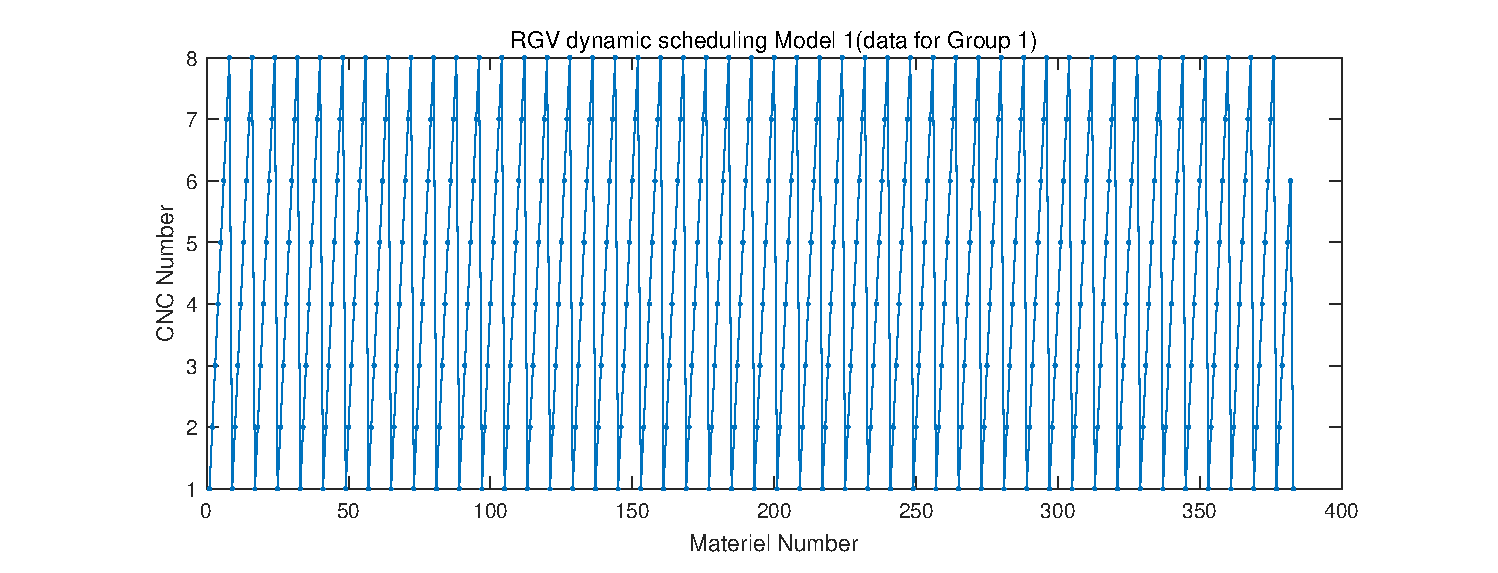
\includegraphics[width=1.07\textwidth]{RGVdynamic1.eps}
	\caption{一道工序情况下RGV动态调度示意图}
     \label{figdy1}
\end{figure}


\noindent(2) 系统的作业效率

在绝对理想的状态下,8个小时内8台CNC永远在工作,没有停歇时间。此时加工物料的总量为:
\begin{equation}
\label{eqst1}
S_t=\dfrac{8\times60\times60\times8}{t_{cnc}}
%=\left\{\begin{array}{ll}
%\left[\dfrac{230400}{560}\right]=411,&\text{第一组数据}\vspace{0.2cm}\\
%\left[\dfrac{230400}{580}\right]=397,&\text{第二组数据}\vspace{0.2cm}\\
%\left[\dfrac{230400}{545}\right]=422,&\text{第三组数据}\\
%\end{array}\right.
\end{equation}

代入3组数据的$t_{cnc}$可得:$$S_{t1}=411,\ S_{t2}=397,\ S_{t3}=422.$$

由模型I计算出的结果,可知一道工序情况下8个小时加工物料的总量为:$$S_{m1}=382,\ S_{m2}=358,\ S_{m3}=391.$$

系统作业效率$\eta$为:
\begin{equation}
\eta=\dfrac{S_m}{S_t}\times100\%,
\end{equation}
代入以上数据可得:$$\eta_1=92.94\%,\ \eta_2=90.18\%,\ \eta_3=92.65\%.$$

\noindent(3) 模型的实用性和算法的有效性

通过对MATLAB输出的数据进行分析可知,RGV是按照CNC1\#至CNC8\#的顺序循环工作的,易知这种状态就是整个系统能够达到的最优状态。所以,虽然我们是通过每次寻找局部最优的方法入手解决问题,但是我们得到的结果已经是全局最优解。

经3组数据检验,模型得出了合理的结论,具有实用性。算法快速有效,系统的作业效率约为92\%,已经达到了全局最优。

\subsection{两道工序情况的分析与求解}

\subsubsection{对任务的分析}

两道工序的物料加工作业情况,每个物料的第一和第二道工序分别由两台不同的CNC依次加工完成。针对此问题,我们首先要确定加工第一道工序的CNC分别是哪几台,同时确定加工第二道工序的CNC是哪几台。RGV首先对加工第一道工序的CNC上料,等待第一道工序结束,将半成品上料到加工第二道工序的CNC,然后大致重复此流程。RGV具体的动态调度采取寻找当前最优解的贪心算法策略。

\subsubsection{对任务的求解}

\noindent{\bfseries\song 模型II—基于贪心算法求解最优动态调度方案模型}

\noindent1. 模型的建立

我们首先进行工序分配,针对三组不同的数据,指定三种不同的工序分配方案:

\vspace{0.4cm}
$\left\{\begin{array}{ll}
1:&\text{第一道工序与第二道工序各自4台CNC}\\
2:&\text{执行第一道工序的CNC数目大于执行第二道工序的CNC数目}\\
3:&\text{执行第一道工序的CNC数目小于执行第二道工序的CNC数目}\\
\end{array}\right.$

\vspace{0.4cm}

定义工序分配集合:
\begin{definition}
三种不同的工序分配方案对应的工序分配集合定义为
$$S_1=\{(4,4)\},\ S_2=\{(5,3),(6,2),(7,1)\},\ S_3=\{(3,5),(2,6),(1,7)\},$$
其中每种情况用一个数对表示,第一个数字表示执行第一道工序的CNC数目,第二个数字表示执行第二道工序的CNC数目。
\end{definition}
%针对三种不同的工序,初步作出如下假设:
%
%\begin{assumption}
%工序分配假设
%
%\vspace{0.3cm}
%
%$\left\{\begin{array}{ll}
%1:&\text{CNC1\#,3\#,5\#,7\#执行第一道工序;CNC2\#,4\#,6\#,8\#执行第二道工序。}\\
%2:&\text{CNC1\#,2\#,3\#,5\#,7\#执行第一道工序;CNC4\#,6\#,8\#执行第二道工序。}\\
%3:&\text{CNC4\#,6\#,8\#执行第一道工序;CNC1\#,2\#,3\#,5\#,7\#执行第二道工序。}\\
%\end{array}\right.$
%\end{assumption}

针对三种不同的工序分配方案,我们对$S_i,\ i=1,2,3,$循环遍历所有可能的情况,确定哪几台CNC执行第一道工序,哪几台CNC执行第二道工序,可以使系统的生产效率达到最优,一共遍历了$C_8^1+C_8^2+\cdots+C_8^7=2^8-2\times1=254$种情况。

虽然工序分配有三种情况,但是RGV的动态调度原则可以统一表述。
%\begin{definition}
记第一道工序包含的CNC编号集合为$P^1$,
%\begin{equation}
%P^1=\left\{\begin{array}{ll}
%\{1,3,5,7\},&\text{若工序分配假设 {\rm1}成立,}\\
%\{1,2,3,5,7\},&\text{若工序分配假设 {\rm2}成立,}\\
%\{4,6,8\},&\text{若工序分配假设 {\rm3}成立.}\\
%\end{array}\right.
%\end{equation}
第二道工序包含的CNC编号集合为$P^2$,
%\begin{equation}
%P^2=\left\{\begin{array}{ll}
%\{2,4,6,8\},&\text{若工序分配假设 {\rm1}成立,}\\
%\{4,6,8\},&\text{若工序分配假设 {\rm2}成立,}\\
%\{1,2,3,5,7\},&\text{若工序分配假设 {\rm3}成立.}\\
%\end{array}\right.
%\end{equation}
%\end{definition}
那么,两道工序情况下RGV的动态调度原则(模型)为:

\begin{principle}
RGV下一步要去的位置$P'$为RGV从当前位置$P=i$行走到$P=j$的时间$\mathbf{T_{rgvm}}(j)$与该位置两台CNC之一加工剩余时间以及RGV给其上下料时间之和最小的位置。$p$为机械爪上是否有熟料标志, {\rm1}表示有, {\rm0}表示无。当$p=0$时,RGV只处理第一道工序CNC发出的请求;当$p=1$时,RGV只处理第二道工序CNC发出的请求。那么,RGV下一步要去的位置$P'$为
\begin{equation}
P'=\left\{\begin{array}{l}
j\Bigg|\min\left\{\begin{array}{ll}
\min\left\{\mathbf{T_{rgvm}}(j)+\mathbf{T_{cncw}}(2j-1)+\mathbf{T_{rgvw}}(2j-1)\}\right\},& if\ 2j-1\in P^1,\\
\min\left\{\mathbf{T_{rgvm}}(j)+\mathbf{T_{cncw}}(2j)+\mathbf{T_{rgvw}}(2j)\}\right\},& if\ 2j\in P^1,\\
\end{array}\right\},\ if\ p=0;\vspace{0.2cm}\\
j\Bigg|\min\left\{\begin{array}{ll}
\min\left\{\mathbf{T_{rgvm}}(j)+\mathbf{T_{cncw}}(2j-1)+\mathbf{T_{rgvw}}(2j-1)\}\right\},& if\ 2j-1\in P^2,\\
\min\left\{\mathbf{T_{rgvm}}(j)+\mathbf{T_{cncw}}(2j)+\mathbf{T_{rgvw}}(2j)\}\right\},& if\ 2j\in P^2,\\
\end{array}\right\},\ if\ p=1.\\
\end{array}\right.
\end{equation}

\end{principle}

\noindent2. 模型的算法

在两道工序的情况下,基于贪心算法求解最优动态调度方案模型的算法如流程图
\ref{pro2}所示。

RGV动态调度的第二个模型主要用于解决不考虑机器故障情况下的两道工序物料作业加工情况。该模型基于贪婪法在每次RGV要执行下一动作时求得对每个设备执行的时间长短并以此来作出选择。由于出现了两道工序,所以最开始需要对所有分组情况进行遍历,得到最大物料数的分组即为最优解。

由于不同的CNC分成了两组,因此通过更改总时间矩阵某些项的大小可以达到先进行第一道工序再进行第二道工序的效果。分组完毕后,根据RGV下一步需要执行的操作来增加相应的操作时间。若即将到达八小时,机器将不再完成上料工作,等待所有下料清洗结束后回到初始状态。此部分在程序中并未体现,需人工去除程序生成的最后几项超时的物料。

\begin{figure}[!htbp]
	\vspace{-1.5cm}
	\hspace{-1cm}
	\includegraphics[width=1.08\textwidth]{floatchart2b.pdf}
	\caption{两道工序基于贪心算法模型的流程图}
     \label{pro2}
\end{figure}

\noindent3. 模型的求解

\noindent(1) RGV的调度策略

通过对$S_i,\ i=1,2,3,$中所有可能情况的遍历,最终确定第一组数据应该采用工序分配方案为(4,4),并且取得最优解的(4,4)的具体分配不唯一,其中一种可行的方案为:第一道工序为CNC1\#, CNC3\#, CNC5\#, CNC7\#;第二道工序为CNC2\#, CNC4\#, CNC6\#, CNC8\#。

第二组应该采用的工序分配方案为(4,4),并且取得最优解的(4,4)的具体分配只有一种:第一道工序为CNC2\#, CNC4\#, CNC6\#, CNC8\#;第二道工序为CNC1\#, CNC3\#, CNC5\#, CNC7\#。

而第三组应该采用的工序分配方案为(5,3),并且取得最优解的(5,3)的具体分配不唯一,其中一种可行的方案为:第一道工序为CNC1\#, CNC3\#, CNC4\#, CNC6\#, CNC8\#;第二道工序为CNC2\#, CNC5\#, CNC7\#。

RGV的调度策略与模型I类似,每一步只寻找下一步的局部最优解,具体表述为原则2。由MATLAB作出第一组数据的RGV动态调度示意图如\ref{figdy2}所示,其他两组数据的图片放在附录。

\begin{figure}[!htbp]
	\hspace{-0.5cm}
	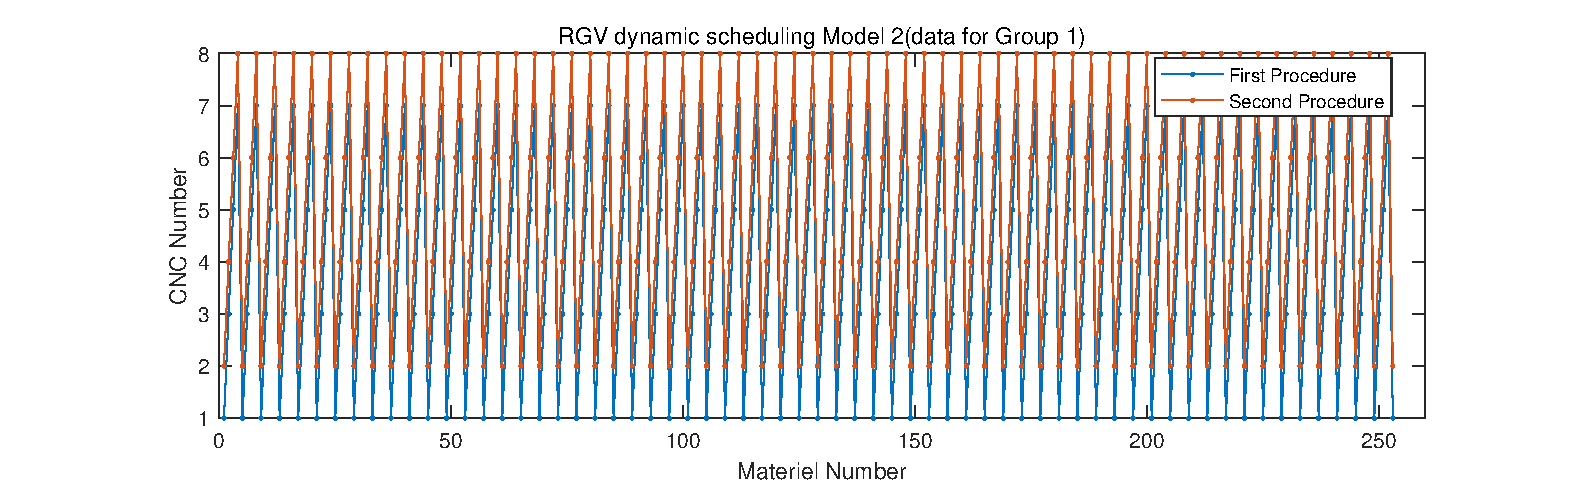
\includegraphics[width=1.07\textwidth]{RGV_dynamic2_1.eps}
	\caption{两道工序情况下RGV动态调度示意图(第一组数据)}
     \label{figdy2}
\end{figure}

\noindent(2) 系统的作业效率

在绝对理想的状态下,8个小时内加工第二道工序的CNC永远在工作,没有停歇时间。代入3组数据可得此时加工物料的总量为:
$$S_{t1}=\dfrac{28800\times4}{t_{cnc2}}=288,
\ S_{t2}=\dfrac{28800\times4}{t_{cnc2}}=230,
\ S_{t3}=\dfrac{28800\times3}{t_{cnc2}}=274.$$

由模型II计算出的结果为:$$S_{m1}=253,\ S_{m2}=210,\ S_{m3}=245.$$

系统作业效率$\eta$为:
$$\eta_1=87.85\%,\ \eta_2=91.30\%,\ \eta_3=89.42\%.$$

\noindent(3) 模型的实用性和算法的有效性

通过对模型结构以及MATLAB输出的数据进行分析可知,模型对3组数据分别给出了相对的最优解,具有实用性。算法快速有效,系统的作业效率约为89\%,已经达到了比较理想的状态。

\subsection{考虑故障概率一道工序与两道工序情况的分析与求解}

\subsubsection{对任务的分析}

CNC在加工过程中以大约1\%的概率发生故障,发生故障时,未完成的物料报废。误工时间介于10到20分钟之间,故障排除后立即加入作业序列。在有CNC发生故障的情况下,RGV需要重新进行动态调度的规划,在剩余的没有发生故障的CNC中寻求最优位置。我们采用模拟退火算法的思想对这种情况进行建模求解。

\subsubsection{对任务的求解}

\noindent{\bfseries\song 模型III—基于模拟退火算法求解最优故障动态调度方案模型:一道工序}

\noindent1. 模型的建立

CNC在加工过程中以大约1\%的概率发生故障的情况下,RGV的动态调度原则与没有故障时相似。为了给出统一的表达式,我们首先定义一个考虑故障时一道工序情况下CNC的剩余工作时间矩阵:

\begin{definition}
一道工序情况下,考虑故障时CNC剩余工作时间矩阵
\begin{equation}
\mathbf{T_{crash}}(i)=\left\{\begin{array}{ll}
\mathbf{T_{cncw}}(i),&\text{若CNCi\#没有发生故障,}\\
t_{cnc},&\text{若CNCi\#发生故障,}\\
\end{array}\right.
,\ i=1,2,\cdots,8.
\end{equation}

当CNCi\#发生故障时,将$\mathbf{T_{crash}}(i)$取为CNC加工完成一个一道工序的物料所需时间$t_{cnc}$, 可以在取最小值时避免取到发生故障的CNCi\#.
\end{definition}

这样我们得到了考虑故障时CNC的剩余工作时间矩阵$\mathbf{T_{crash}}$,将原则1中$\mathbf{T_{cncw}}$换为$\mathbf{T_{crash}}$即可确定考虑故障时在一道工序情况下RGV的动态调度原则(模型)。

\begin{principle}
RGV下一步要去的位置$P'$为RGV从当前位置$P=i$行走到$P=j$的时间$\mathbf{T_{rgvm}}(j)$与$\min\{\mathbf{T_{crash}}(2j-1)+\mathbf{T_{rgvw}}(2j-1),\mathbf{T_{crash}}(2j)+\mathbf{T_{rgvw}}(2j)\}$之和最小的位置,即
\begin{equation}
P'=j\Big|\min\left\{\mathbf{T_{rgvm}}(j)+\min\{\mathbf{T_{crash}}(2j-1)+\mathbf{T_{rgvw}}(2j-1),\mathbf{T_{crash}}(2j)+\mathbf{T_{rgvw}}(2j)\}\right\},\ \ i, j=1,2,3,4.
\end{equation}

\end{principle}

\noindent2. 模型的算法

考虑故障时,一道工序情况下基于模拟退火算法求解最优动态调度方案模型的算法如流程图\ref{pro3}所示。

RGV动态调度的第三个模型主要用于解决可能发生机器故障的一道工序物料作业加工情况。该模型利用贪婪法求出RGV下一步进行操作的最短路径,为了保证可以找到更加优化的解,该模型在生成最短路径时采用了模拟退火算法,一定概率寻找倒数第二短的路径并执行相应操作。

根据对总时间矩阵的判定选择路径。选择完毕后根据RGV下一步需要执行的操作来增加相应的操作时间。每给机器上一次料就进行一次故障检测,若无故障则按照原来的规则继续运行,若有故障,则生成一个故障发生的时间以及人工维护需要的时间(利用均匀分布),然后重新计算总时间矩阵选择最优路径。若即将到达八小时,机器将不再完成上料工作,等待所有下料清洗结束后回到初始状态。此部分在程序中并未体现,需人工去除程序生成的最后几项超时的物料。

\begin{figure}[!htbp]
	\vspace{-1.3cm}
	\hspace{-1.5cm}
	\includegraphics[width=1.2\textwidth]{floatchart3b.pdf}
	\caption{考虑故障时一道工序模拟退火模型的流程图}
     \label{pro3}
\end{figure}

\noindent3. 模型的求解

\noindent(1) RGV的调度策略

RGV的调度策略为:通过模拟退火算法每一步基于原则3的思想寻找当前最优解,并且有一定概率寻找倒数第二短的路径,多次运行以寻求全局最优解,然后RGV按照最优解的路线移动。由MATLAB作出第一组数据的RGV动态调度示意图如\ref{figdy3}所示,其他两组数据的图片放在附录。

\begin{figure}[!htbp]
	\hspace{-0.5cm}
	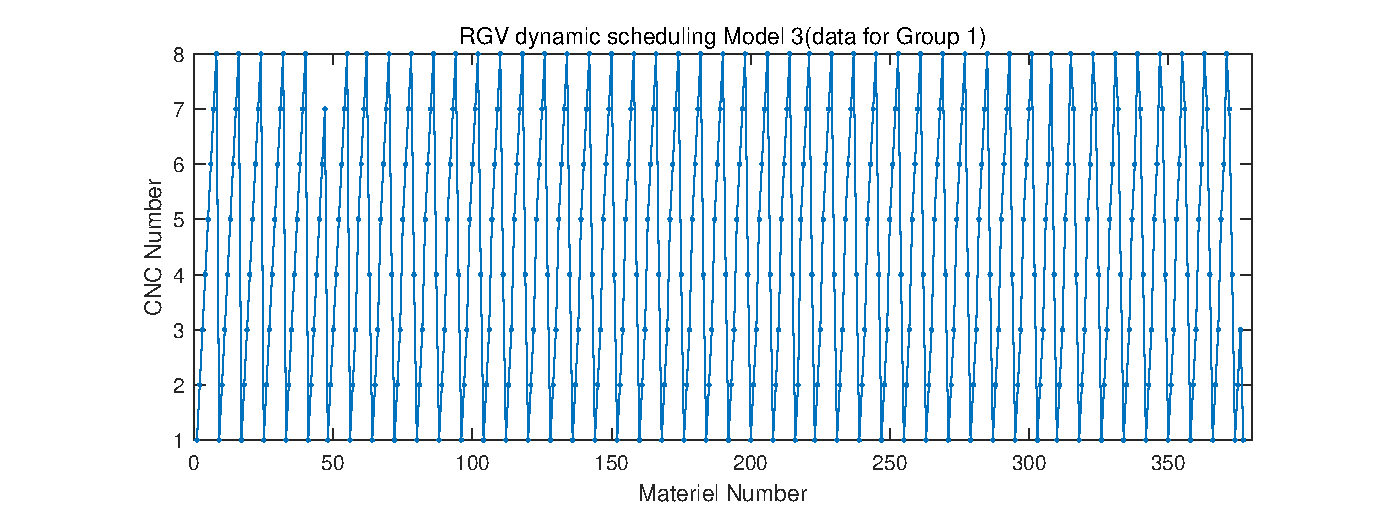
\includegraphics[width=1.07\textwidth]{RGV_dynamic3_1.eps}
	\caption{考虑故障时一道工序情况下RGV动态调度示意图(第一组数据)}
     \label{figdy3}
\end{figure}

\noindent(2) 系统的作业效率

在绝对理想的状态下,8个小时内加工第二道工序的CNC永远在工作,不会发生故障,没有停歇时间。根据模型I中得出的公式(\ref{eqst1})可知此时加工物料的总量与模型I相同,为:
$$S_{t1}=411,
\ S_{t2}=397,
\ S_{t3}=422.$$

由模型III计算出的结果,可知一道工序情况下考虑故障时8个小时加工物料的总量为:$$S_{m1}=372,\ S_{m2}=343,\ S_{m3}=385.$$

系统作业效率$\eta$为:
$$\eta_1=90.51\%,\ \eta_2=86.40\%,\ \eta_3=91.23\%.$$

\noindent(3) 模型的实用性和算法的有效性

经数据检验,模型得出的结果基本符合有故障情况下智能加工系统的工作状态,但是由于试验样本较小,故障概率并未完全符合1\%。总的来说,模型合理地模拟了智能加工系统中有CNC会发生故障的情况,具有实用性。算法快速有效,较好的实现了有故障发生时RGV的动态调度,系统的作业效率约为89\%,已经达到了比较理想的状态。

\noindent{\bfseries\song 模型IV—基于模拟退火算法求解最优故障动态调度方案模型:两道工序}

\noindent1. 模型的建立

在模型III中已经寻找到针对三组不同数据的最佳工序分配方案,模型IV延续此方案并对模型III的思想进行推广。

定义一个考虑故障时两道工序情况下CNC的剩余工作时间矩阵$\mathbf{T'_{crash}}$:

\begin{definition}
两道工序情况下,考虑故障时CNC剩余工作时间矩阵
\begin{equation}
\mathbf{T'_{crash}}(i)=\left\{\begin{array}{ll}
\mathbf{T_{cncw}}(i),&\text{若CNCi\#没有发生故障,}\\
t_{cnc1},&\text{若CNCi\#发生故障,且}\,i\in P^1,\\
t_{cnc2},&\text{若CNCi\#发生故障,且}\,i\in P^2,\\
\end{array}\right.
\ i=1,2,\cdots,8.
\end{equation}

当CNCi\#发生故障时,将$\mathbf{T_{crash}}(i)$取为CNC加工完成一个第一道工序的物料所需时间$t_{cnc1}$或加工完成一个第二道工序的物料所需的时间$t_{cnc2}$, 可以在取最小值时避免取到发生故障的CNCi\#.
\end{definition}

考虑故障时,两道工序情况下RGV的动态调度原则(模型)可以建立如下:

\begin{principle}
RGV下一步要去的位置$P'$为RGV从当前位置$P=i$行走到$P=j$的时间$\mathbf{T_{rgvm}}(j)$与该位置两台CNC之一加工剩余时间以及RGV给其上下料时间之和最小的位置。$p$为机械爪上是否有熟料标志, {\rm1}表示有, {\rm0}表示无。当$p=0$时,RGV只处理第一道工序CNC发出的请求;当$p=1$时,RGV只处理第二道工序CNC发出的请求。那么,RGV下一步要去的位置$P'$为
\begin{equation}
P'=\left\{\begin{array}{l}
j\Bigg|\min\left\{\begin{array}{ll}
\min\left\{\mathbf{T_{rgvm}}(j)+\mathbf{T_{crash}}(2j-1)+\mathbf{T_{rgvw}}(2j-1)\}\right\},& if\ 2j-1\in P^1,\\
\min\left\{\mathbf{T_{rgvm}}(j)+\mathbf{T_{crash}}(2j)+\mathbf{T_{rgvw}}(2j)\}\right\},& if\ 2j\in P^1,\\
\end{array}\right\},\ if\ p=0;\\
j\Bigg|\min\left\{\begin{array}{ll}
\min\left\{\mathbf{T_{rgvm}}(j)+\mathbf{T_{crash}}(2j-1)+\mathbf{T_{rgvw}}(2j-1)\}\right\},& if\ 2j-1\in P^2,\\
\min\left\{\mathbf{T_{rgvm}}(j)+\mathbf{T_{crash}}(2j)+\mathbf{T_{rgvw}}(2j)\}\right\},& if\ 2j\in P^2,\\
\end{array}\right\},\ if\ p=1.\\
\end{array}\right.
\end{equation}

\end{principle}

\noindent2. 模型的算法

考虑故障时,两道工序情况下基于模拟退火算法求解最优动态调度方案模型的算法如流程图\ref{pro4}所示。

RGV动态调度的第四个模型主要用于解决可能发生机器故障情况下的两道工序物料作业加工情况。该模型利用贪心算法求出RGV下一步进行操作的最短路径。由于机器有损坏的可能,因此为了找到更优化的解,该模型在生成最短路径时采用了模拟退火算法,一定概率寻找倒数第二短的路径并执行相应操作。由第二个模型的结果可以得到对第四个模型三种情况的最佳分组。

由于不同的CNC分成两道工序,因此需要对总时间矩阵根据不同情况作出相应的修改以符合模型的实际情况。当得出下一步需要进行的操作以及操作位置时,根据相应的操作来增加相应的操作时间,当给一个机器(无论是第一道工序的机器还是第二道工序的机器)进行上料操作时,对这个机器进行一次故障检测,若有故障,则通过一定的概率模型生成此次故障发生的具体时间以及人工需要维护的时间(利用均匀分布),然后重新计算总时间矩阵选择最优路径。若即将到达八小时,机器将不再完成上料工作,等待所有下料清洗结束后回到初始状态。此部分在程序中并未体现,需人工去除程序生成的最后几项超时的物料。

\begin{figure}[!htbp]
	\vspace{-1.5cm}
	\hspace{-0.5cm}
	\includegraphics[width=1.08\textwidth]{floatchart4b.pdf}
	\caption{考虑故障时两道工序模拟退火模型的流程图}
     \label{pro4}
\end{figure}

\noindent3. 模型的求解

\noindent(1) RGV的调度策略

RGV的调度策略为:通过模拟退火算法,每一步基于原则4的思想寻找当前最优解,并且有一定概率寻找倒数第二短的路径,多次运行以寻求全局最优解,然后RGV按照最优解的路线移动。由MATLAB作出第一组数据的RGV动态调度示意图如\ref{figdy4}所示,其他两组数据的图片放在附录。

\begin{figure}[!htbp]
	\hspace{-0.5cm}
	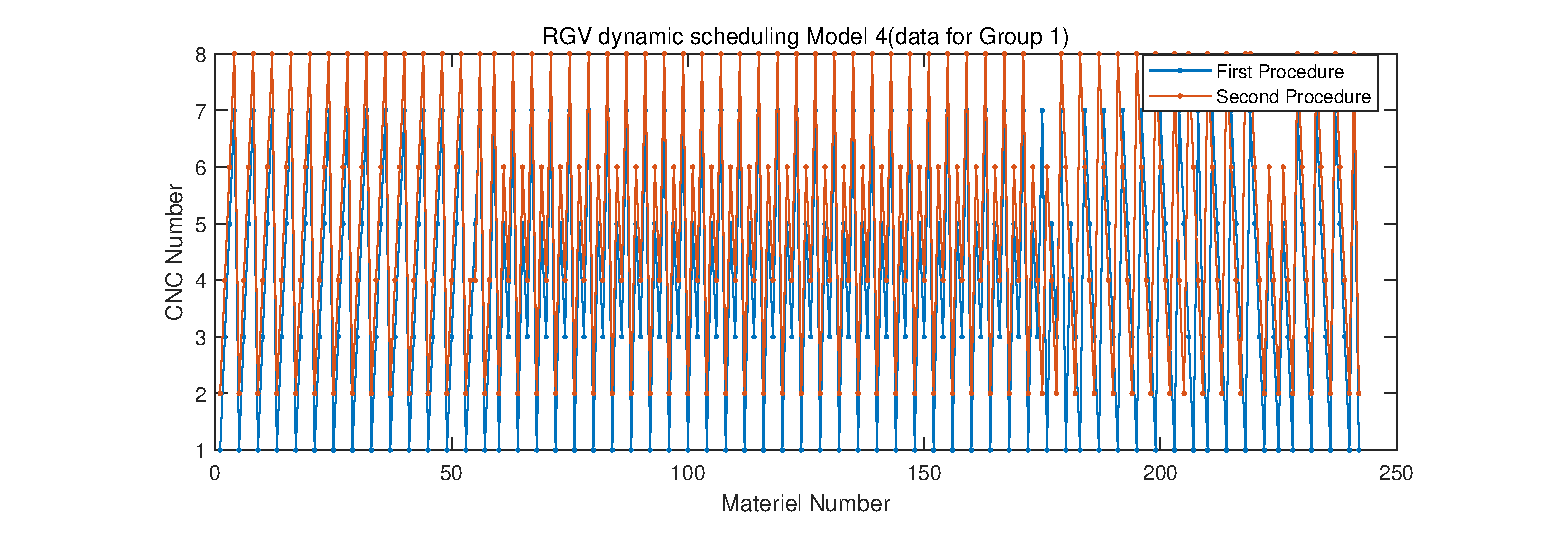
\includegraphics[width=1.07\textwidth]{RGV_dynamic4_1.eps}
	\caption{考虑故障时两道工序情况下RGV动态调度示意图(第一组数据)}
     \label{figdy4}
\end{figure}

\noindent(2) 系统的作业效率

在绝对理想的状态下,8个小时内加工第二道工序的CNC永远在工作,没有停歇时间。代入3组数据可得此时加工物料的总量为:
$$S_{t1}=\dfrac{28800\times4}{t_{cnc2}}=288,
\ S_{t2}=\dfrac{28800\times4}{t_{cnc2}}=230,
\ S_{t3}=\dfrac{28800\times3}{t_{cnc2}}=274.$$

由模型IV计算出的结果,可知考虑故障时两道工序情况下8个小时加工的物料总量为:$$S_{m1}=237,\ S_{m2}=198,\ S_{m3}=238.$$

系统作业效率$\eta$为:
$$\eta_1=82.29\%,\ \eta_2=86.09\%,\ \eta_3=86.86\%.$$

\noindent(3) 模型的实用性和算法的有效性

经数据检验,模型合理地模拟了智能加工系统中考虑CNC会发生故障时两道工序的情况,具有实用性。算法快速有效,较好的实现了有故障发生时两道工序情况下RGV的动态调度,系统的作业效率约为85\%,已经达到了比较理想的状态。

\section{模型的仿真}

FlexSim是一个基于Windows的,面向对象的仿真环境,用于建立离散事件流程,例如制造业,物料处理和办公室工作流,这些全都配以相似度极高的三维虚拟现实环境。

由于时间有限,我们使用FlexSim只对本问题不考虑故障时一道工序的情况进行仿真,仿真中间过程如图\ref{figsim}所示。

\begin{figure}[!htbp]
	\centering
	\includegraphics[width=0.8\textwidth]{simmulation.png}
	\caption{智能加工系统仿真模拟图}
     \label{figsim}
\end{figure}

得到的结果与用MATLAB计算模型I得出的结果一致。

\section{误差分析与灵敏度分析}
\subsection{误差分析}

1. 模型III和模型IV采用模拟退火算法寻找全局最优解,但是概率值的设定会对是否能够找到最优解有较大的影响,所以我们得到的不一定是全局最优解。即我们给出的结果与最优解之间可能存在误差。

2. CNC发生故障后会停止工作10至20分钟,称为误工时间。我们对这段时间的处理是采用均匀分布随机生成一个10到20分钟的数作为误工时间,然而实际情况下,误工时间的分布可能是正态分布,泊松分布,超几何分布等。误工时间与实际情况可能存在误差。

\subsection{灵敏度分析}

将题目中所给3组数据中两道工序的时间比例进行扩展分析,设定两道工序总时长为800秒,分别设定五个不同的比例:200:600, 300:500, 400:400, 500:300, 600:200, 对模型进行灵敏度分析,如图\ref{figsen}所示。图中,横坐标1表示工序分配方案为(4,4),2表示工序分配方案为(5,3),3表示工序分配方案为(3,5),可以发现不同的两道工序时间比例对应的最佳工序分配方案可能会有差异,模型对此反应很灵敏。
\begin{figure}[!htbp]
	\centering
	\includegraphics[width=0.8\textwidth]{sensitivity.eps}
	\caption{灵敏度分析}
     \label{figsen}
\end{figure}

\section{模型的评价与推广}
\subsection{模型的评价}
\subsubsection{模型的优点}

1、模型I以非常简单的贪心算法的思想就寻找到了全局最优解,简捷高效

2、模型II创新性地设置了机械爪上是否有熟料的标志变量,使得模型的数学表达式简洁优美;并且模型II遍历了所有可能的工序分配方案,可以处理所有不同的工序时间比例情况,具有通用性和普适性

3、模型III创新性地定义了一道工序情况下考虑故障时CNC剩余工作时间矩阵,使得模型的数学表达式非常简洁;并且模型III采用了模拟退火算法以弥补贪心算法可能陷入局部最优解的缺点,使得寻找到全局最优解的可能性大大提高。

4、模型IV创新性地定义了两道工序情况下考虑故障时CNC剩余工作时间矩阵,使得模型IV的表达式与模型III可以统一为一个简洁的形式;并且模型IV对故障的模拟非常符合实际情况,使得模型的实用性大大增强。

\subsubsection{模型的缺点}

1、由于每班次连续作业8小时,作业结束时RGV需要回到原位,并且不能有未结束加工的CNC,所以模型需要进行作业结束处理。这里我们采用人工对最后不能完成加工的CNC提前进行关机处理,没有完全实现自动化控制。

2、模型采用的模拟退火算法不能保证一定能够寻找到全局最优解。

\subsection{模型的推广}

{\bfseries\song1.基于贪心算法求解最优动态调度方案模型的推广}

基于贪心算法,我们设计了求解不考虑故障时,一道工序与两道工序情况下RGV的动态调度模型。事实上,该模型还可以解决多道工序情况下贪心算法还可以解决RGV的动态调度问题,以及类似情境下如仓库中往返存取货物等问题。并且,贪心算法还可以用来解决单源最短路径问题,最小生成树问题等。

{\bfseries\song2.基于模拟退火算法求解最优故障动态调度方案模型的推广}

基于模拟退火算法,我们设计了考虑故障时,一道工序与两道工序情况下RGV的动态调度模型。事实上,该模型还可以推广到广泛应用于自动化立体仓库系统中搬运物料的穿梭车上。并且,模拟退火算法还可以用于VLSI设计、图像识别和神经网计算机的研究等。

\section{模型的改进}
本文在寻找最优路径的时候使用了模拟退火算法,但是模拟退火算法不能保证一定能够寻找到全局最优解。全局优化算法又称现代启发式算法,是一种具有全局优化性能、通用性强且适合于并行处理的算法。全局优化算法不止有模拟退火算法,还有遗传算法 、禁忌搜索算法、粒子群算法、蚁群算法等。为了增大寻找到全局最优解的概率,可以使用不同的全局优化算法分别建模计算,比较所得结果,选取最优化的动态调度方案。

\newpage
%参考文献
\begin{thebibliography}{9}%宽度9
 \bibitem{bib:one} Dotoli M, Fanti M P. A colored Petri net model for automated storage and retrieval systems serviced by rail-guided vehicles: a control perspective [J]. International Journal of Computer Integrated Manufacturing, 2005, 18(2-3): 122-136.
 \bibitem{bib:two} Chen F F, Huang J, Centeno M.A. Intelligent scheduling and control of rail-guided vehicles and load/unload operations in a flexible manufacturing system[J]. Journal of Intelligent Manufacturing, 1999, 10(5): 405-421. 
 \bibitem{bib:three} 吴长庆, 罗键, 陈火国等. 基于Petri网的RGV系统中环路死锁研究[J]. 计算机科学, 2009, 36(4): 250-253.
 \bibitem{bib:four} 陈华, 孙启元. 基于TS算法的直线往复2-RGV系统调度研究[J]. 工业工程与管理,   2015, 20(05): 80-88.
\bibitem{bib:five} 杨少华, 张家毅, 赵立. 基于排队论的环轨多车数量与能力分析[J]. 制造业自动化, 2011, 33(16): 102-104.
\bibitem{bib:six} 吴焱明, 刘永强, 张栋等. 基于遗传算法的RGV动态调度研究[J]. 起重运输机械, 2012(06): 20-23.
\bibitem{bib:seven}卓金武, 李必文, 魏永生等. MATLAB 在数学建模中的应用[M], 北京:北京 航空航天大学出版社, 2014.
\bibitem{bib:eight}龚纯, 王正林. 精通 MATLAB 最优化计算[M], 北京: 电子工业出版社, 2012.
\bibitem{bib:nine}姜启源, 谢金星, 叶俊. 数学模型[M], 北京: 高等教育出版社, 2003.
\end{thebibliography}

\newpage
%附录
\appendix
\renewcommand{\thefigure}{\Alph{section}-\arabic{figure}}
\section{RGV动态仿真示意图}

\begin{figure}[H]
	\hspace{-0.5cm}
	\includegraphics[width=1.07\textwidth]{RGV_dynamic2_2.eps}
	\caption{两道工序情况下RGV动态调度示意图(第二组数据)}
\end{figure}

\begin{figure}[H]
	\hspace{-0.5cm}
	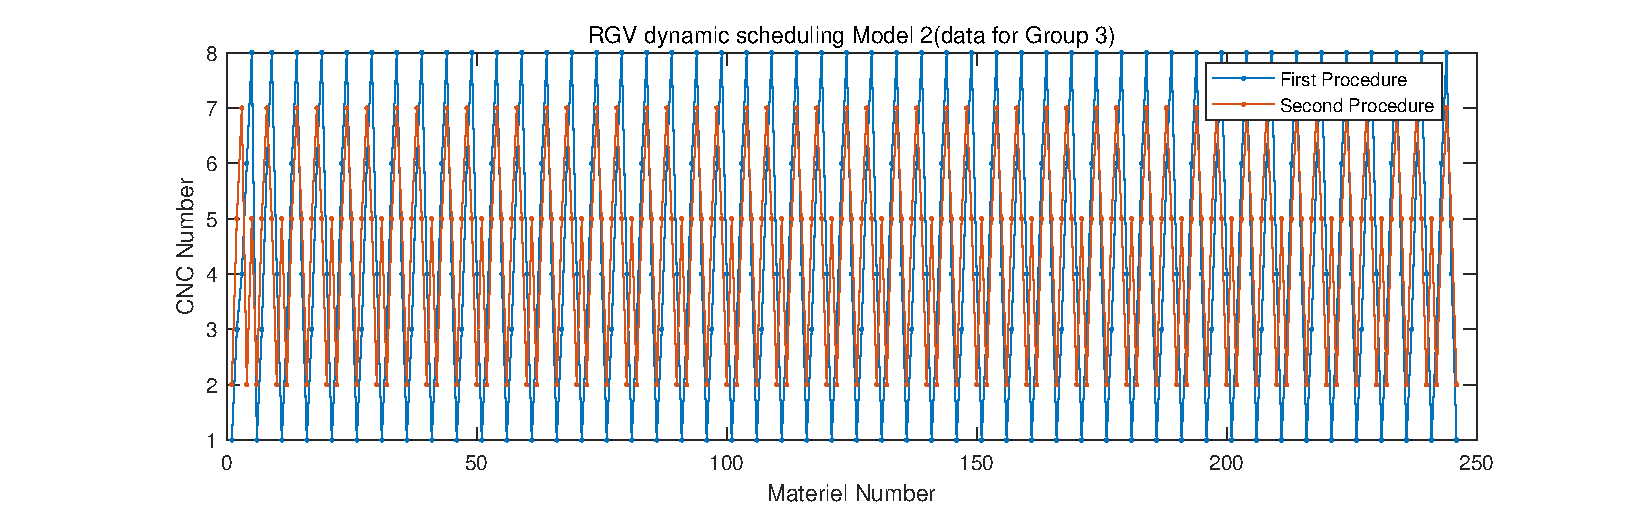
\includegraphics[width=1.07\textwidth]{RGV_dynamic2_3.eps}
	\caption{两道工序情况下RGV动态调度示意图(第三组数据)}
\end{figure}

\begin{figure}[H]
	\hspace{-0.5cm}
	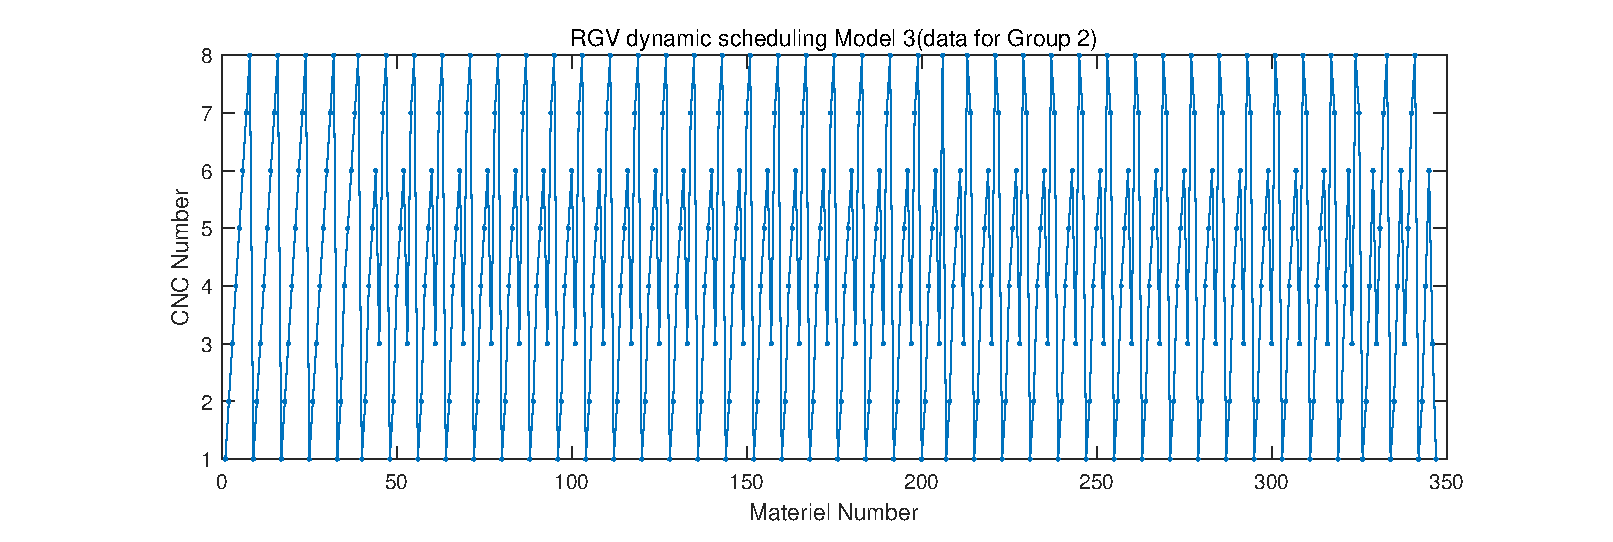
\includegraphics[width=1.07\textwidth]{RGV_dynamic3_2.eps}
	\caption{考虑故障时一道工序情况下RGV动态调度示意图(第二组数据)}
\end{figure}

\begin{figure}[H]
	\hspace{-0.5cm}
	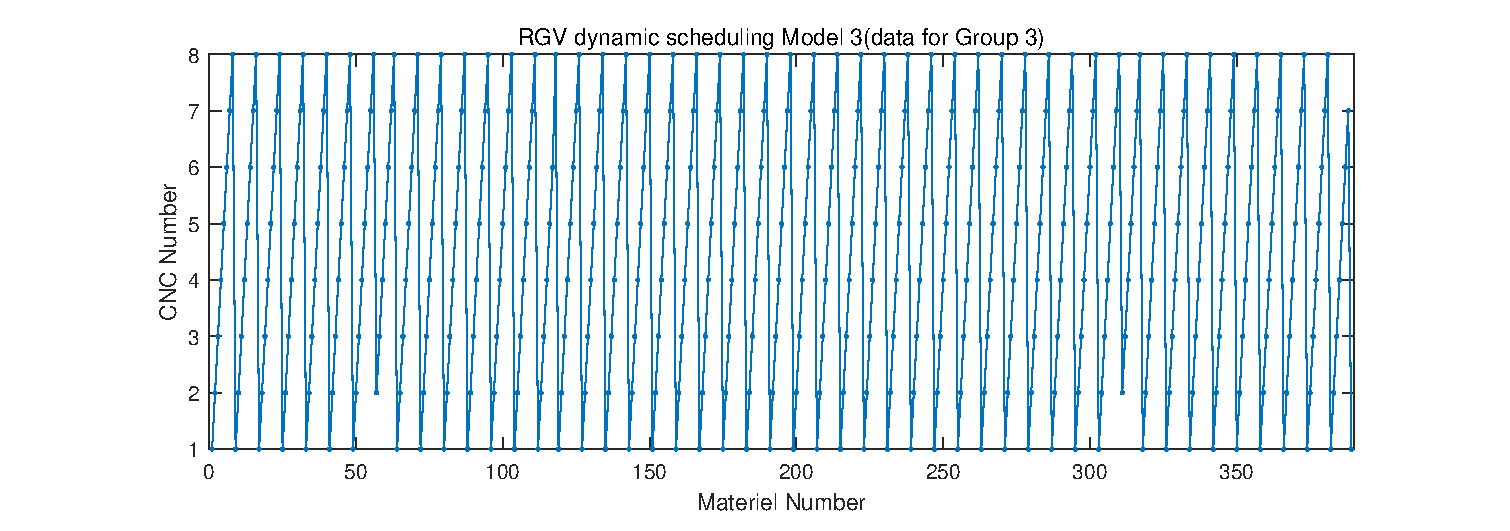
\includegraphics[width=1.07\textwidth]{RGV_dynamic3_3.eps}
	\caption{考虑故障时一道工序情况下RGV动态调度示意图(第三组数据)}
\end{figure}

\begin{figure}[H]
	\hspace{-0.5cm}
	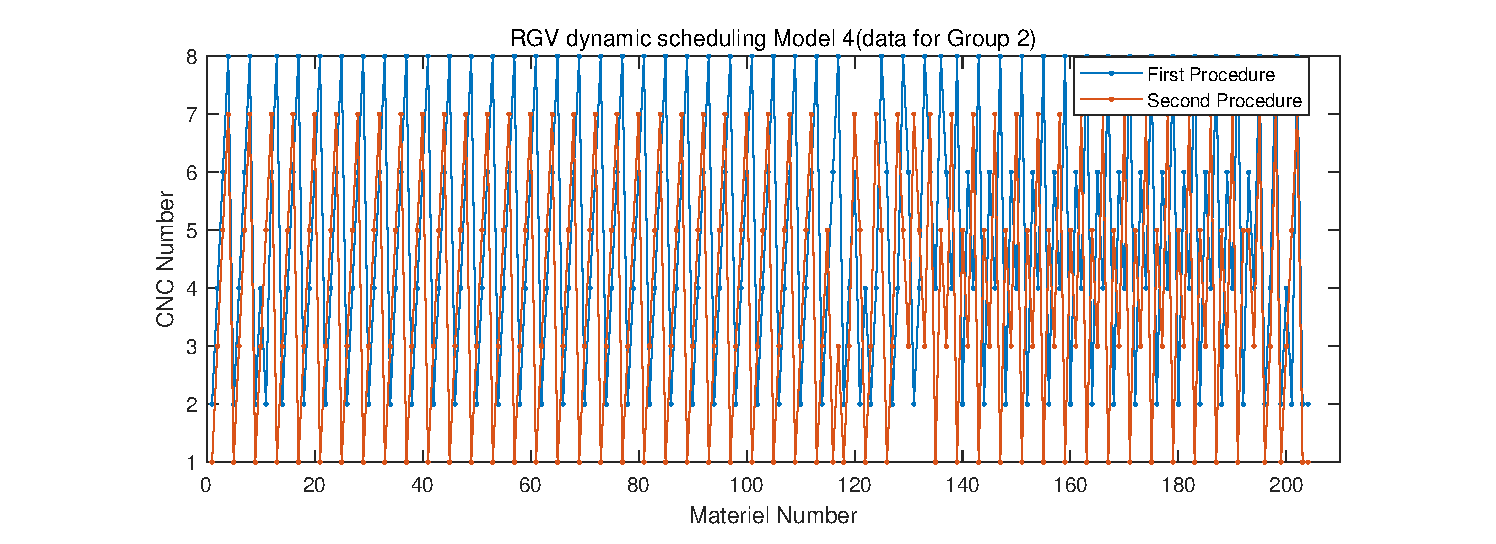
\includegraphics[width=1.07\textwidth]{RGV_dynamic4_2.eps}
	\caption{考虑故障时两道工序情况下RGV动态调度示意图(第二组数据)}
\end{figure}

\begin{figure}[H]
	\hspace{-0.5cm}
	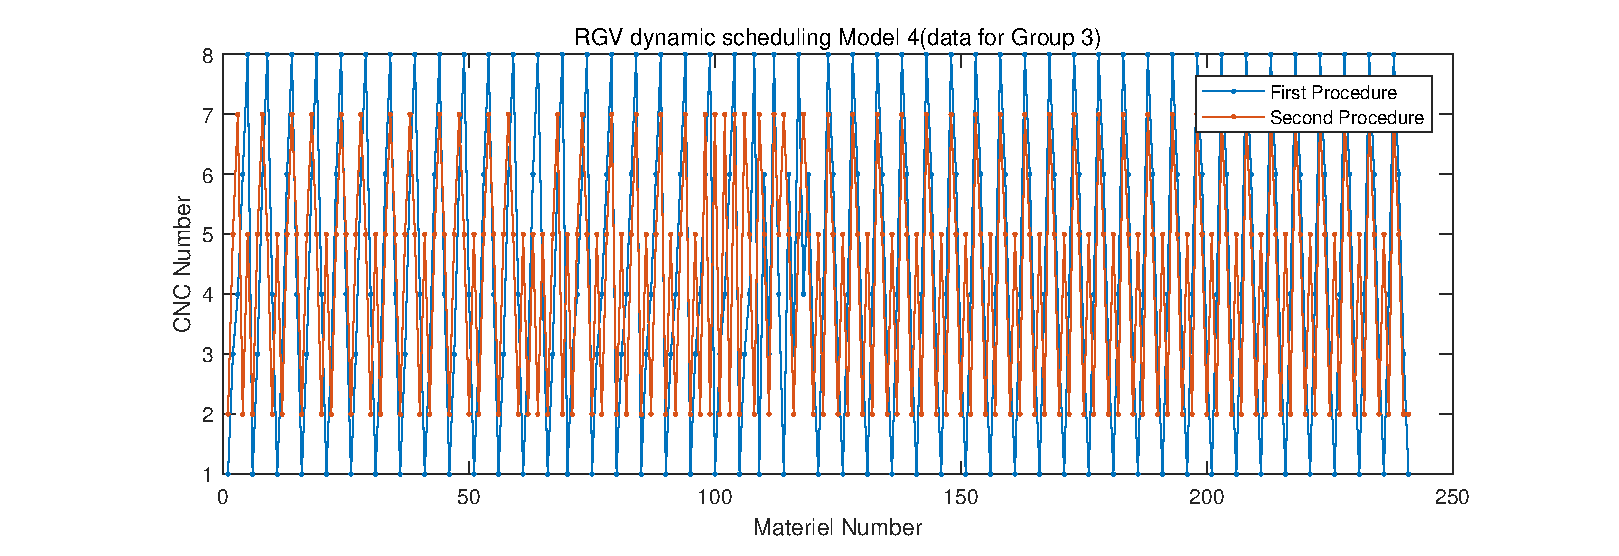
\includegraphics[width=1.07\textwidth]{RGV_dynamic4_3.eps}
	\caption{考虑故障时两道工序情况下RGV动态调度示意图(第三组数据)}
\end{figure}

\newpage

\section{ 一道工序(无故障)--MATLAB 源程序}
\begin{lstlisting}[language=matlab]
%   初始化MATLAB
clear
clc

%   数据初始化
%   第一组数据
tm1 = 20;                       %   RGV移动1个单位时间
tm2 = 33;                       %   RGV移动2个单位时间
tm3 = 46;                       %   RGV移动3个单位时间
tcnc = 560;                     %   CNC加工完成一道工序时间
trwo = 28;                      %   RGV为奇数CNC上下料时间
trwe = 31;                      %   RGV为偶数CNC上下料时间
tclr = 25;                      %   RGV清洗熟料时间
%   第二组数据
%tm1 = 23;                       %   RGV移动1个单位时间
%tm2 = 41;                       %   RGV移动2个单位时间
%tm3 = 59;                       %   RGV移动3个单位时间
%tcnc = 580;                     %   CNC加工完成一道工序时间
%trwo = 30;                      %   RGV为奇数CNC上下料时间
%trwe = 35;                      %   RGV为偶数CNC上下料时间
%tclr = 30;                      %   RGV清洗熟料时间
%   第三组数据
%tm1 = 18;                       %   RGV移动1个单位时间
%tm2 = 32;                       %   RGV移动2个单位时间
%tm3 = 46;                       %   RGV移动3个单位时间
%tcnc = 545;                     %   CNC加工完成一道工序时间
%trwo = 27;                      %   RGV为奇数CNC上下料时间
%trwe = 32;                      %   RGV为偶数CNC上下料时间
%tclr = 25;                      %   RGV清洗熟料时间
Twork = 28800;                  %   总工作时间
CNCnum = 8;                     %   CNC机器数
t = 0;                          %   时间初始化
Pos = 1;                        %   位置初始化
CNCw = zeros(1, CNCnum);        %   CNC工作状态标志
Trgvm = zeros(1, CNCnum);       %   RGV移动时间矩阵
Trgvw = zeros(1, CNCnum);       %   RGV工作时间矩阵
Tcncw = zeros(1, CNCnum);       %   CNC工作时间矩阵
Ttotal = zeros(1, CNCnum);      %   总时间矩阵
paw = 0;                        %   机械爪上是否有熟料
Tclear = 100000;                %   清洗剩余时间
tmin = 10000;                   %   循环变量,表示当前步骤进行的最短时间
minPos = -1;                    %   循环变量,表示当前对哪台机器操作
count = zeros(1, CNCnum);       %   计算每台机器所上料的数目
starttime = zeros(50, CNCnum); %   每台机器上料所对应的时间
endtime = zeros(50, CNCnum);   %   每台机器下料对应时间
TotalProduct = 0;               %   总的物料产量

while t < Twork
    %   根据RGV当前位置计算对应的RGV移动时间矩阵
    switch Pos
        case 1
            Trgvm(1) = 0;
          	Trgvm(2) = 0;
            Trgvm(3) = tm1;
           	Trgvm(4) = tm1;
         	Trgvm(5) = tm2;
           	Trgvm(6) = tm2;
          	Trgvm(7) = tm3;
           	Trgvm(8) = tm3;
       	case 2
           	Trgvm(1) = tm1;
           	Trgvm(2) = tm1;
         	Trgvm(3) = 0;
          	Trgvm(4) = 0;
           	Trgvm(5) = tm1;
          	Trgvm(6) = tm1;
           	Trgvm(7) = tm2;
           	Trgvm(8) = tm2;               
        case 3
           	Trgvm(1) = tm2;
          	Trgvm(2) = tm2;
          	Trgvm(3) = tm1;
         	Trgvm(4) = tm1;
          	Trgvm(5) = 0;
           	Trgvm(6) = 0;
          	Trgvm(7) = tm1;
           	Trgvm(8) = tm1;
     	case 4
         	Trgvm(1) = tm3;
          	Trgvm(2) = tm3;
           	Trgvm(3) = tm2;
          	Trgvm(4) = tm2;
           	Trgvm(5) = tm1;
          	Trgvm(6) = tm1;
        	Trgvm(7) = 0;
           	Trgvm(8) = 0;        
    end
    %   计算RGV工作时间矩阵
	Trgvw(1) = trwo;
	Trgvw(3) = trwo;
    Trgvw(5) = trwo;
	Trgvw(7) = trwo;
	Trgvw(2) = trwe;
	Trgvw(4) = trwe;
	Trgvw(6) = trwe;
	Trgvw(8) = trwe;
    %   计算总时间
    Ttotal = Trgvm + Trgvw + Tcncw;
    %   生成最短路径位置及时间
    [tmin, minPos] = min(Ttotal);
    %   若机械爪上有熟料,则将熟料清洗时间算入
    if paw == 1
        Tclear = tclr;
    else
        Tclear = 100000;
    end
    %   若最短时间大于清洗时间,则先进行清洗
    if tmin > Tclear
        t = t + tclr;
        Tcncw(CNCw == 1) = Tcncw(CNCw == 1) - tclr;
        paw = paw - 1;
    %   若需要操作的设备不在当前位置,则移动
    elseif ceil(minPos/2) ~= Pos
        Pos = ceil(minPos/2);
        t = t + Trgvm(minPos);
        Tcncw(CNCw == 1) = Tcncw(CNCw == 1) - Trgvm(minPos);
    %   若需要操作的位置在当前设备
    else
        %   若当前设备未工作,进行上料操作并计数
        if CNCw(minPos) == 0
            count(minPos) = count(minPos) + 1;
            starttime(count(minPos), minPos) = t;
            t = t + Trgvw(minPos);
            Tcncw(CNCw == 1) = Tcncw(CNCw == 1) - Trgvw(minPos);
            Tcncw(Tcncw<0) = 0;
            Tcncw(minPos) = Tcncw(minPos) + tcnc;
            CNCw(minPos) = 1;
        %   若当前设备正在工作
        else
            %   若设备已工作完毕,进行下料操作并计数
            if Tcncw(minPos) == 0
                endtime(count(minPos), minPos) = t;
                count(minPos) = count(minPos) + 1;
                starttime(count(minPos), minPos) = t;
                t = t + Trgvw(minPos);
                paw = paw + 1;
                Tcncw(CNCw == 1) = Tcncw(CNCw == 1) - Trgvw(minPos);
                Tcncw(Tcncw<0) = 0;
                Tcncw(minPos) = Tcncw(minPos) + tcnc;
                CNCw(minPos) = 1;
            %   若设备正在工作,等待
            else 
                t = t + 1;
                Tcncw(CNCw == 1) = Tcncw(CNCw == 1) - 1;
            end
        end
    end
    %   去除小于0的数
    Tcncw(Tcncw<0) = 0;
end

%   数据输出

%   由于最后快接近八小时的时候需要停止某些机器和RGV的上下料操作以保证能在八小时
%   内进行设备停止并回到初始位置,因此程序计算结果需经进一步人工处理才能得到
%   真正的值,所以程序生成的数据和导入Excel表格中的数据会有微小误差

%   判断每个产出物料是否有效
Logiccount = endtime > 0;
%   输出每个物料上料时间,其中矩阵的行为不同的物料,列为在哪个CNC机器上
starttime
%   输出每个物料下料时间,其中矩阵的行为不同的物料。列为在哪个机器上
endtime
%   输出总产量
TotalProduct = sum(Logiccount(:))
\end{lstlisting}

\section{ 两道工序(第1组数据,无故障)--MATLAB 源程序}
\begin{lstlisting}[language=matlab]
%   MATLAB初始化
clear
clc

%   由于第二个模型加工物料需要两道工序,因此需要考虑CNC如何进行分组,每组
%   分配多少个CNC的问题。在这里先进行按照(4,4)、(3,5)、(5,3)的分组结构
%   进行循环遍历,发现(4,4)分组的某一种方式得到的物料最多,因此给出(4,4)
%   分组如何遍历,以及遍历完毕后输出最优解。而(3,5)分组遍历在程序结束后的
%   注释给出。(5,3)分组遍历只需将相应的第一道工序和第二道工序对调即可。

%   通过计算得到,第一道工序CNC序号为1,3,5,7;第二道工序CNC序号为2,4,6,8
%   (最优解不唯一)

%   数据初始化
load('firstgroup4.mat');
all = [1, 2, 3, 4, 5, 6, 7, 8];
groupcount = zeros(70, 1);
secondgroup = zeros(70, 4);

%   对(4,4)分组的每种情况进行遍历
for divgroup = 1: 70
    %   得到第二道工序的CNC序号
    secondgroup(divgroup,:) = setdiff(all, firstgroup(divgroup,:));
    tm1 = 20;                       %   RGV移动1个单位时间
    tm2 = 33;                       %   RGV移动2个单位时间
    tm3 = 46;                       %   RGV移动3个单位时间
    tcnc1 = 400;                    %   CNC完成第一道工序所需时间
    tcnc2 = 378;                    %   CNC完成第二道工序所需时间
    trwo = 28;                      %   RGV为奇数CNC上下料时间
    trwe = 31;                      %   RGV为偶数CNC上下料时间
    tclr = 25;                      %   RGV清洗熟料时间
    Twork = 28800;                  %   总工作时间
    CNCnum = 8;                     %   CNC机器数
    t = 0;                          %   时间初始化
    Pos = 1;                        %   位置初始化
    CNCw = zeros(1, CNCnum);        %   CNC工作状态标志
    Trgvm = zeros(1, CNCnum);      	%   RGV移动时间矩阵
    Trgvw = zeros(1, CNCnum);       %   RGV工作时间矩阵
    Tcncw = zeros(1, CNCnum);       %   CNC工作时间矩阵
    Ttotal = zeros(1, CNCnum);      %   总时间矩阵
    pawsecond = 0;                  %   需要进行第二道工序的物料
    pawclear = 0;                   %   需要清洗的物料
    Tclear = 100000;                %   清洗剩余时间
    count1 = zeros(1, CNCnum);      %   计算每台机器第一道工序上料数目
    count2 = zeros(1, CNCnum);      %   计算每台机器第二道工序上料数目
    starttime1 = zeros(70, CNCnum);%   每台机器第一道工序上料所对应时间
    starttime2 = zeros(70, CNCnum);%   每台机器第二道工序上料所对应时间
    endtime1 = zeros(70, CNCnum);  %   每台机器第一道工序下料所对应时间
    endtime2 = zeros(70, CNCnum);  %   每台机器第二道工序下料所对应时间
    
    %   总时间不超过8小时
    while t < Twork
        %   根据RGV所在位置计算RGV移动时间矩阵
        switch Pos
            case 1
                Trgvm(1) = 0;
                Trgvm(2) = 0;
                Trgvm(3) = tm1;
                Trgvm(4) = tm1;
                Trgvm(5) = tm2;
                Trgvm(6) = tm2;
                Trgvm(7) = tm3;
                Trgvm(8) = tm3;
            case 2
                Trgvm(1) = tm1;
                Trgvm(2) = tm1;
                Trgvm(3) = 0;
                Trgvm(4) = 0;
                Trgvm(5) = tm1;
                Trgvm(6) = tm1;
                Trgvm(7) = tm2;
                Trgvm(8) = tm2;               
            case 3
                Trgvm(1) = tm2;
                Trgvm(2) = tm2;
                Trgvm(3) = tm1;
                Trgvm(4) = tm1;
                Trgvm(5) = 0;
                Trgvm(6) = 0;
                Trgvm(7) = tm1;
                Trgvm(8) = tm1;
            case 4
                Trgvm(1) = tm3;
                Trgvm(2) = tm3;
                Trgvm(3) = tm2;
                Trgvm(4) = tm2;
                Trgvm(5) = tm1;
                Trgvm(6) = tm1;
                Trgvm(7) = 0;
                Trgvm(8) = 0;        
        end
        %   根据RGV要对设备进行的操作计算RGV工作时间矩阵
        Trgvw(1) = trwo;
        Trgvw(3) = trwo;
        Trgvw(5) = trwo;
        Trgvw(7) = trwo;
        Trgvw(2) = trwe;
        Trgvw(4) = trwe;
        Trgvw(6) = trwe;
        Trgvw(8) = trwe;
        %   若暂时没有第一道工序加工完成的半成品,则第二道工序对应机器暂停
        if pawsecond == 0
            Trgvw(secondgroup(divgroup, 1)) = ...
                Trgvw(secondgroup(divgroup, 1)) + 100000;
            Trgvw(secondgroup(divgroup, 2)) = ...
                Trgvw(secondgroup(divgroup, 2)) + 100000;
            Trgvw(secondgroup(divgroup, 3)) = ...
                Trgvw(secondgroup(divgroup, 3)) + 100000;
            Trgvw(secondgroup(divgroup, 4)) = ...
                Trgvw(secondgroup(divgroup, 4)) + 100000;
        else
            Trgvw(firstgroup(divgroup, 1)) = ...
                Trgvw(firstgroup(divgroup, 1)) + 100000;
            Trgvw(firstgroup(divgroup, 2)) = ...
                Trgvw(firstgroup(divgroup, 2)) + 100000;
            Trgvw(firstgroup(divgroup, 3)) = ...
                Trgvw(firstgroup(divgroup, 3)) + 100000;
            Trgvw(firstgroup(divgroup, 4)) = ...
                Trgvw(firstgroup(divgroup, 4)) + 100000;
        end
        %   计算总时间矩阵
        Ttotal = Trgvm + Trgvw + Tcncw;
        %   计算下一步最短时间及路径
        [tmin, minPos] = min(Ttotal);
        %   若机械爪上有待清洗的熟料,计算清洗时间
        if pawclear > 0
            Tclear = tclr;
        else
            Tclear = 100000;
        end
        %   若下一步最短路径所对应时间大于清洗时间,先进行清洗操作
        if tmin > Tclear
            t = t + tclr;
            Tcncw(CNCw == 1) = Tcncw(CNCw == 1) - tclr;
            pawclear = pawclear - 1;
        %   若下一步要操作的对象不在此处,则移动RGV
        elseif ceil(minPos/2) ~= Pos
            Pos = ceil(minPos/2);
            t = t + Trgvm(minPos);
            Tcncw(CNCw == 1) = Tcncw(CNCw == 1) - Trgvm(minPos);
        %   若下一步要操作的对向在此处
        else
            switch minPos
                %   若操作对象为第一道工序CNC
                case {firstgroup(divgroup, 1), firstgroup(divgroup, 2), ...
                        firstgroup(divgroup, 3), firstgroup(divgroup, 4)}
                    %   若操作对象未开始工作,进行上料处理并计数
                    if CNCw(minPos) == 0
                        count1(minPos) = count1(minPos) + 1;
                        starttime1(count1(minPos), minPos) = t;
                        t = t + Trgvw(minPos);
                        Tcncw(CNCw == 1) = Tcncw(CNCw == 1) - Trgvw(minPos);
                        Tcncw(Tcncw<0) = 0;
                        Tcncw(minPos) = Tcncw(minPos) + tcnc1;
                        CNCw(minPos) = 1;
                    %   若操作对象的工作状态标记为1
                    else
                        %   若操作对象已工作完毕,则先下料再上料并计数
                        if Tcncw(minPos) == 0
                            endtime1(count1(minPos), minPos) = t;
                            count1(minPos) = count1(minPos) + 1;
                            starttime1(count1(minPos), minPos) = t;
                            t = t + Trgvw(minPos);
                            pawsecond = pawsecond + 1;
                            Tcncw(CNCw == 1) = Tcncw(CNCw == 1) - Trgvw(minPos);
                            Tcncw(Tcncw<0) = 0;
                            Tcncw(minPos) = Tcncw(minPos) + tcnc1;
                            CNCw(minPos) = 1;
                        %   若操作对象未工作完毕,则等待
                        else
                            t = t + 1;
                            Tcncw(CNCw == 1) = Tcncw(CNCw == 1) - 1;
                        end
                    end
                %   若操作对象为第二道工序CNC
                case {secondgroup(divgroup, 1), secondgroup(divgroup, 2), ...
                        secondgroup(divgroup, 3), secondgroup(divgroup, 4)}
                    %   若操作对象未开始工作,上料并计数
                    if CNCw(minPos) == 0
                        count2(minPos) = count2(minPos) + 1;
                        starttime2(count2(minPos), minPos) = t;
                        t = t + Trgvw(minPos);
                        Tcncw(CNCw == 1) = Tcncw(CNCw == 1) - Trgvw(minPos);
                        Tcncw(Tcncw<0) = 0;
                        Tcncw(minPos) = Tcncw(minPos) + tcnc2;
                        CNCw(minPos) = 1;
                        pawsecond = pawsecond - 1;
                    %   若操作对象工作状态标记为1
                    else
                        %   若操作对象已工作完毕,则先下料再上料并计数
                        if Tcncw(minPos) == 0
                            endtime2(count2(minPos), minPos) = t;
                            count2(minPos) = count2(minPos) + 1;
                            starttime2(count2(minPos), minPos) = t;
                            t = t + Trgvw(minPos);
                            pawclear = pawclear + 1;
                            Tcncw(CNCw == 1) = Tcncw(CNCw == 1) - Trgvw(minPos);
                            Tcncw(Tcncw<0) = 0;
                            Tcncw(minPos) = Tcncw(minPos) + tcnc2;
                            CNCw(minPos) = 1;
                            pawsecond = pawsecond - 1;
                        %   若操作对象未工作完毕,则等待
                        else
                            t = t + 1;
                            Tcncw(CNCw == 1) = Tcncw(CNCw == 1) - 1;
                        end
                    end
            end
        end
        Tcncw(Tcncw<0) = 0;
    end
    %   计算每种情况所生产的物料数
    logiccount = endtime2 > 0;
    groupcount(divgroup) = sum(logiccount(:));
end

%   找出能生产出最大物料的组合方式
[Totalcount, divgroup] = max(groupcount);
%   重新计算每个物料的第一道和第二道工序的上料和下料时间
%   得到第二道工序的CNC序号
secondgroup(divgroup,:) = setdiff(all, firstgroup(divgroup,:));
tm1 = 20;                       %   RGV移动1个单位时间
tm2 = 33;                       %   RGV移动2个单位时间
tm3 = 46;                       %   RGV移动3个单位时间
tcnc1 = 400;                    %   CNC完成第一道工序所需时间
tcnc2 = 378;                    %   CNC完成第二道工序所需时间
trwo = 28;                      %   RGV为奇数CNC上下料时间
trwe = 31;                      %   RGV为偶数CNC上下料时间
tclr = 25;                      %   RGV清洗熟料时间
Twork = 28800;                  %   总工作时间
CNCnum = 8;                     %   CNC机器数
t = 0;                          %   时间初始化
Pos = 1;                        %   位置初始化
CNCw = zeros(1, CNCnum);        %   CNC工作状态标志
Trgvm = zeros(1, CNCnum);      	%   RGV移动时间矩阵
Trgvw = zeros(1, CNCnum);       %   RGV工作时间矩阵
Tcncw = zeros(1, CNCnum);       %   CNC工作时间矩阵
Ttotal = zeros(1, CNCnum);      %   总时间矩阵
pawsecond = 0;                  %   需要进行第二道工序的物料
pawclear = 0;                   %   需要清洗的物料
Tclear = 100000;                %   清洗剩余时间
count1 = zeros(1, CNCnum);      %   计算每台机器第一道工序上料数目
count2 = zeros(1, CNCnum);      %   计算每台机器第二道工序上料数目
starttime1 = zeros(70, CNCnum);%   每台机器第一道工序上料所对应时间
starttime2 = zeros(70, CNCnum);%   每台机器第二道工序上料所对应时间
endtime1 = zeros(70, CNCnum);  %   每台机器第一道工序下料所对应时间
endtime2 = zeros(70, CNCnum);  %   每台机器第二道工序下料所对应时间

%   总时间不超过8小时
while t < Twork
    %   根据RGV所在位置计算RGV移动时间矩阵
    switch Pos
        case 1
            Trgvm(1) = 0;
            Trgvm(2) = 0;
            Trgvm(3) = tm1;
            Trgvm(4) = tm1;
            Trgvm(5) = tm2;
            Trgvm(6) = tm2;
            Trgvm(7) = tm3;
            Trgvm(8) = tm3;
        case 2
            Trgvm(1) = tm1;
            Trgvm(2) = tm1;
            Trgvm(3) = 0;
            Trgvm(4) = 0;
            Trgvm(5) = tm1;
            Trgvm(6) = tm1;
            Trgvm(7) = tm2;
            Trgvm(8) = tm2;               
        case 3
            Trgvm(1) = tm2;
            Trgvm(2) = tm2;
            Trgvm(3) = tm1;
            Trgvm(4) = tm1;
            Trgvm(5) = 0;
            Trgvm(6) = 0;
            Trgvm(7) = tm1;
            Trgvm(8) = tm1;
        case 4
            Trgvm(1) = tm3;
            Trgvm(2) = tm3;
            Trgvm(3) = tm2;
            Trgvm(4) = tm2;
            Trgvm(5) = tm1;
            Trgvm(6) = tm1;
            Trgvm(7) = 0;
            Trgvm(8) = 0;        
    end
    %   根据RGV要对设备进行的操作计算RGV工作时间矩阵
    Trgvw(1) = trwo;
    Trgvw(3) = trwo;
    Trgvw(5) = trwo;
    Trgvw(7) = trwo;
    Trgvw(2) = trwe;
    Trgvw(4) = trwe;
    Trgvw(6) = trwe;
    Trgvw(8) = trwe;
    %   若暂时没有第一道工序加工完成的半成品,则第二道工序对应机器暂停
    if pawsecond == 0
        Trgvw(secondgroup(divgroup, 1)) = Trgvw(secondgroup(divgroup, 1)) + 100000;
        Trgvw(secondgroup(divgroup, 2)) = Trgvw(secondgroup(divgroup, 2)) + 100000;
        Trgvw(secondgroup(divgroup, 3)) = Trgvw(secondgroup(divgroup, 3)) + 100000;
        Trgvw(secondgroup(divgroup, 4)) = Trgvw(secondgroup(divgroup, 4)) + 100000;
    else
        Trgvw(firstgroup(divgroup, 1)) = Trgvw(firstgroup(divgroup, 1)) + 100000;
        Trgvw(firstgroup(divgroup, 2)) = Trgvw(firstgroup(divgroup, 2)) + 100000;
        Trgvw(firstgroup(divgroup, 3)) = Trgvw(firstgroup(divgroup, 3)) + 100000;
        Trgvw(firstgroup(divgroup, 4)) = Trgvw(firstgroup(divgroup, 4)) + 100000;
    end
    %   计算总时间矩阵
    Ttotal = Trgvm + Trgvw + Tcncw;
    %   计算下一步最短时间及路径
    [tmin, minPos] = min(Ttotal);
    %   若机械爪上有待清洗的熟料,计算清洗时间
    if pawclear > 0
        Tclear = tclr;
    else
        Tclear = 100000;
    end
    %   若下一步最短路径所对应时间大于清洗时间,先进行清洗操作
    if tmin > Tclear
        t = t + tclr;
        Tcncw(CNCw == 1) = Tcncw(CNCw == 1) - tclr;
        pawclear = pawclear - 1;
    %   若下一步要操作的对象不在此处,则移动RGV
    elseif ceil(minPos/2) ~= Pos
        Pos = ceil(minPos/2);
        t = t + Trgvm(minPos);
        Tcncw(CNCw == 1) = Tcncw(CNCw == 1) - Trgvm(minPos);
    %   若下一步要操作的对向在此处
    else
        switch minPos
            %   若操作对象为第一道工序CNC
            case {firstgroup(divgroup, 1), firstgroup(divgroup, 2), ...
                    firstgroup(divgroup, 3), firstgroup(divgroup, 4)}
                %   若操作对象未开始工作,进行上料处理并计数
                if CNCw(minPos) == 0
                    count1(minPos) = count1(minPos) + 1;
                    starttime1(count1(minPos), minPos) = t;
                    t = t + Trgvw(minPos);
                    Tcncw(CNCw == 1) = Tcncw(CNCw == 1) - Trgvw(minPos);
                    Tcncw(Tcncw<0) = 0;
                    Tcncw(minPos) = Tcncw(minPos) + tcnc1;
                    CNCw(minPos) = 1;
                %   若操作对象的工作状态标记为1
                else
                    %   若操作对象已工作完毕,则先下料再上料并计数
                    if Tcncw(minPos) == 0
                        endtime1(count1(minPos), minPos) = t;
                        count1(minPos) = count1(minPos) + 1;
                        starttime1(count1(minPos), minPos) = t;
                        t = t + Trgvw(minPos);
                        pawsecond = pawsecond + 1;
                        Tcncw(CNCw == 1) = Tcncw(CNCw == 1) - Trgvw(minPos);
                        Tcncw(Tcncw<0) = 0;
                        Tcncw(minPos) = Tcncw(minPos) + tcnc1;
                        CNCw(minPos) = 1;
                    %   若操作对象未工作完毕,则等待
                    else
                        t = t + 1;
                        Tcncw(CNCw == 1) = Tcncw(CNCw == 1) - 1;
                    end
                end
            %   若操作对象为第二道工序CNC
            case {secondgroup(divgroup, 1), secondgroup(divgroup, 2), ...
                    secondgroup(divgroup, 3), secondgroup(divgroup, 4)}
                %   若操作对象未开始工作,上料并计数
                if CNCw(minPos) == 0
                    count2(minPos) = count2(minPos) + 1;
                    starttime2(count2(minPos), minPos) = t;
                    t = t + Trgvw(minPos);
                    Tcncw(CNCw == 1) = Tcncw(CNCw == 1) - Trgvw(minPos);
                    Tcncw(Tcncw<0) = 0;
                    Tcncw(minPos) = Tcncw(minPos) + tcnc2;
                    CNCw(minPos) = 1;
                    pawsecond = pawsecond - 1;
                %   若操作对象工作状态标记为1
                else
                    %   若操作对象已工作完毕,则先下料再上料并计数
                    if Tcncw(minPos) == 0
                        endtime2(count2(minPos), minPos) = t;
                        count2(minPos) = count2(minPos) + 1;
                        starttime2(count2(minPos), minPos) = t;
                        t = t + Trgvw(minPos);
                        pawclear = pawclear + 1;
                        Tcncw(CNCw == 1) = Tcncw(CNCw == 1) - Trgvw(minPos);
                        Tcncw(Tcncw<0) = 0;
                        Tcncw(minPos) = Tcncw(minPos) + tcnc2;
                        CNCw(minPos) = 1;
                        pawsecond = pawsecond - 1;
                    %   若操作对象未工作完毕,则等待
                    else
                        t = t + 1;
                        Tcncw(CNCw == 1) = Tcncw(CNCw == 1) - 1;
                    end
                end
        end
    end
    Tcncw(Tcncw<0) = 0;
end    

%   数据输出

%   由于最后快接近八小时的时候需要停止某些机器和RGV的上下料操作以保证能在八小时
%   内进行设备停止并回到初始位置,因此程序计算结果需经进一步人工处理才能得到
%   真正的值,所以程序生成的数据和导入Excel表格中的数据会有微小误差

%   判断每个产出物料是否有效
logiccount = endtime2 > 0;
%   输出每个物料上料时间,其中矩阵的行为不同的物料,列为在哪个CNC机器上
%   分第一道工序和第二道工序
starttime1
starttime2
%   输出每个物料下料时间,其中矩阵的行为不同的物料。列为在哪个机器上
%   分第一道工序和第二道工序
endtime1
endtime2
%   输出总产量
TotalProduct = sum(logiccount(:))





% %   若为(3,5)分组,遍历代码
% %   MATLAB初始化
% clear
% clc
% 
% %   数据初始化
% load('firstgroup3.mat');
% all = [1, 2, 3, 4, 5, 6, 7, 8];
% groupcount = zeros(70, 1);
% secondgroup = zeros(70, 5);
% 
% 
% for divgroup = 1: 56
%     secondgroup(divgroup,:) = setdiff(all, firstgroup3(divgroup,:));
%     tm1 = 20;                       %   RGV移动1个单位时间
%     tm2 = 33;                       %   RGV移动2个单位时间
%     tm3 = 46;                       %   RGV移动3个单位时间
%     tcnc1 = 400;                    %   CNC完成第一道工序所需时间
%     tcnc2 = 378;                    %   CNC完成第二道工序所需时间
%     trwo = 28;                      %   RGV为奇数CNC上下料时间
%     trwe = 31;                      %   RGV为偶数CNC上下料时间
%     tclr = 25;                      %   RGV清洗熟料时间
%     Twork = 28800;                  %   总工作时间
%     CNCnum = 8;                     %   CNC机器数
%     t = 0;                          %   时间初始化
%     Pos = 1;                        %   位置初始化
%     CNCw = zeros(1, CNCnum);        %   CNC工作状态标志
%     Trgvm = zeros(1, CNCnum);      	%   RGV移动时间矩阵
%     Trgvw = zeros(1, CNCnum);       %   RGV工作时间矩阵
%     Tcncw = zeros(1, CNCnum);       %   CNC工作时间矩阵
%     Ttotal = zeros(1, CNCnum);      %   总时间矩阵
%     pawsecond = 0;                  %   需要进行第二道工序的物料
%     pawclear = 0;                   %   需要清洗的物料
%     Tclear = 100000;                %   清洗剩余时间
%     count1 = zeros(1, CNCnum);      %   计算每台机器第一道工序上料数目
%     count2 = zeros(1, CNCnum);      %   计算每台机器第二道工序上料数目
%     starttime1 = zeros(100, CNCnum);%   每台机器第一道工序上料所对应时间
%     starttime2 = zeros(100, CNCnum);%   每台机器第二道工序上料所对应时间
%     endtime1 = zeros(100, CNCnum);  %   每台机器第一道工序下料所对应时间
%     endtime2 = zeros(100, CNCnum);  %   每台机器第二道工序下料所对应时间
%     %   总时间不超过8小时
%     while t < Twork
%         %   根据RGV所在位置计算RGV移动时间矩阵
%         switch Pos
%             case 1
%                 Trgvm(1) = 0;
%                 Trgvm(2) = 0;
%                 Trgvm(3) = tm1;
%                 Trgvm(4) = tm1;
%                 Trgvm(5) = tm2;
%                 Trgvm(6) = tm2;
%                 Trgvm(7) = tm3;
%                 Trgvm(8) = tm3;
%             case 2
%                 Trgvm(1) = tm1;
%                 Trgvm(2) = tm1;
%                 Trgvm(3) = 0;
%                 Trgvm(4) = 0;
%                 Trgvm(5) = tm1;
%                 Trgvm(6) = tm1;
%                 Trgvm(7) = tm2;
%                 Trgvm(8) = tm2;               
%             case 3
%                 Trgvm(1) = tm2;
%                 Trgvm(2) = tm2;
%                 Trgvm(3) = tm1;
%                 Trgvm(4) = tm1;
%                 Trgvm(5) = 0;
%                 Trgvm(6) = 0;
%                 Trgvm(7) = tm1;
%                 Trgvm(8) = tm1;
%             case 4
%                 Trgvm(1) = tm3;
%                 Trgvm(2) = tm3;
%                 Trgvm(3) = tm2;
%                 Trgvm(4) = tm2;
%                 Trgvm(5) = tm1;
%                 Trgvm(6) = tm1;
%                 Trgvm(7) = 0;
%                 Trgvm(8) = 0;        
%         end
%         %   根据RGV要对设备进行的操作计算RGV工作时间矩阵
%         Trgvw(1) = trwo;
%         Trgvw(3) = trwo;
%         Trgvw(5) = trwo;
%         Trgvw(7) = trwo;
%         Trgvw(2) = trwe;
%         Trgvw(4) = trwe;
%         Trgvw(6) = trwe;
%         Trgvw(8) = trwe;
%         %   若暂时没有第一道工序加工完成的半成品,则第二道工序对应机器暂停
%         if pawsecond == 0
%             Trgvw(secondgroup(divgroup, 1)) = Trgvw(secondgroup(divgroup, 1)) + 100000;
%             Trgvw(secondgroup(divgroup, 2)) = Trgvw(secondgroup(divgroup, 2)) + 100000;
%             Trgvw(secondgroup(divgroup, 3)) = Trgvw(secondgroup(divgroup, 3)) + 100000;
%             Trgvw(secondgroup(divgroup, 4)) = Trgvw(secondgroup(divgroup, 4)) + 100000;
%             Trgvw(secondgroup(divgroup, 5)) = Trgvw(secondgroup(divgroup, 5)) + 100000;
%         else
%             Trgvw(firstgroup3(divgroup, 1)) = Trgvw(firstgroup3(divgroup, 1)) + 100000;
%             Trgvw(firstgroup3(divgroup, 2)) = Trgvw(firstgroup3(divgroup, 2)) + 100000;
%             Trgvw(firstgroup3(divgroup, 3)) = Trgvw(firstgroup3(divgroup, 3)) + 100000;
%         end
%         %   计算总时间矩阵
%         Ttotal = Trgvm + Trgvw + Tcncw;
%         %   计算下一步最短时间及路径
%         [tmin, minPos] = min(Ttotal);
%         %   若机械爪上有待清洗的熟料,计算清洗时间
%         if pawclear > 0
%             Tclear = tclr;
%         else
%             Tclear = 100000;
%         end
%         %   若下一步最短路径所对应时间大于清洗时间,先进行清洗操作
%         if tmin > Tclear
%             t = t + tclr;
%             Tcncw(CNCw == 1) = Tcncw(CNCw == 1) - tclr;
%             pawclear = pawclear - 1;
%         %   若下一步要操作的对象不在此处,则移动RGV
%         elseif ceil(minPos/2) ~= Pos
%             Pos = ceil(minPos/2);
%             t = t + Trgvm(minPos);
%             Tcncw(CNCw == 1) = Tcncw(CNCw == 1) - Trgvm(minPos);
%         %   若下一步要操作的对向在此处
%         else
%             switch minPos
%                 %   若操作对象为第一道工序CNC
%                 case {firstgroup3(divgroup, 1), firstgroup3(divgroup, 2), ...
%                         firstgroup3(divgroup, 3)}
%                     %   若操作对象未开始工作,进行上料处理并计数
%                     if CNCw(minPos) == 0
%                         count1(minPos) = count1(minPos) + 1;
%                         starttime1(count1(minPos), minPos) = t;
%                         t = t + Trgvw(minPos);
%                         Tcncw(CNCw == 1) = Tcncw(CNCw == 1) - Trgvw(minPos);
%                         Tcncw(Tcncw<0) = 0;
%                         Tcncw(minPos) = Tcncw(minPos) + tcnc1;
%                         CNCw(minPos) = 1;
%                     %   若操作对象的工作状态标记为1
%                     else
%                         %   若操作对象已工作完毕,则先下料再上料并计数
%                         if Tcncw(minPos) == 0
%                             endtime1(count1(minPos), minPos) = t;
%                             count1(minPos) = count1(minPos) + 1;
%                             starttime1(count1(minPos), minPos) = t;
%                             t = t + Trgvw(minPos);
%                             pawsecond = pawsecond + 1;
%                             Tcncw(CNCw == 1) = Tcncw(CNCw == 1) - Trgvw(minPos);
%                             Tcncw(Tcncw<0) = 0;
%                             Tcncw(minPos) = Tcncw(minPos) + tcnc1;
%                             CNCw(minPos) = 1;
%                         %   若操作对象未工作完毕,则等待
%                         else
%                             t = t + 1;
%                             Tcncw(CNCw == 1) = Tcncw(CNCw == 1) - 1;
%                         end
%                     end
%                 %   若操作对象为第二道工序CNC
%                 case {secondgroup(divgroup, 1), secondgroup(divgroup, 2), ...
%                         secondgroup(divgroup, 3), secondgroup(divgroup, 4), ...
%                         secondgroup(divgroup, 5)}
%                     %   若操作对象未开始工作,上料并计数
%                     if CNCw(minPos) == 0
%                         count2(minPos) = count2(minPos) + 1;
%                         starttime2(count2(minPos), minPos) = t;
%                         t = t + Trgvw(minPos);
%                         Tcncw(CNCw == 1) = Tcncw(CNCw == 1) - Trgvw(minPos);
%                         Tcncw(Tcncw<0) = 0;
%                         Tcncw(minPos) = Tcncw(minPos) + tcnc2;
%                         CNCw(minPos) = 1;
%                         pawsecond = pawsecond - 1;
%                     %   若操作对象工作状态标记为1
%                     else
%                         %   若操作对象已工作完毕,则先下料再上料并计数
%                         if Tcncw(minPos) == 0
%                             endtime2(count2(minPos), minPos) = t;
%                             count2(minPos) = count2(minPos) + 1;
%                             starttime2(count2(minPos), minPos) = t;
%                             t = t + Trgvw(minPos);
%                             pawclear = pawclear + 1;
%                             Tcncw(CNCw == 1) = Tcncw(CNCw == 1) - Trgvw(minPos);
%                             Tcncw(Tcncw<0) = 0;
%                             Tcncw(minPos) = Tcncw(minPos) + tcnc2;
%                             CNCw(minPos) = 1;
%                             pawsecond = pawsecond - 1;
%                         %   若操作对象未工作完毕,则等待
%                         else
%                             t = t + 1;
%                             Tcncw(CNCw == 1) = Tcncw(CNCw == 1) - 1;
%                         end
%                     end
%             end
%         end
%         Tcncw(Tcncw<0) = 0;
%     end
%     logiccount = endtime2 > 0;
%     groupcount(divgroup) = sum(logiccount(:));
% end
% %   找出能生产出最大物料的组合方式
% [Totalcount, divgroup] = max(groupcount);
\end{lstlisting}

\section{ 两道工序(第2组数据,无故障)--MATLAB 源程序}
\begin{lstlisting}[language=matlab]
%   MATLAB初始化
clear
clc

%   由于第二个模型加工物料需要两道工序,因此需要考虑CNC如何进行分组,每组
%   分配多少个CNC的问题。在这里先进行按照(4,4)、(3,5)、(5,3)的分组结构
%   进行循环遍历,发现(4,4)分组的某一种方式得到的物料最多,因此给出(4,4)
%   分组如何遍历,以及遍历完毕后输出最优解。而(3,5)分组和(5,3)分组遍历
%   参见CUMCM2018BModel2_1.m

%   通过计算得到,第一道工序CNC序号为2,4,6,8;第二道工序CNC序号为1,3,5,7
%   (最优解唯一)

%   数据初始化
load('firstgroup4.mat');
all = [1, 2, 3, 4, 5, 6, 7, 8];
groupcount = zeros(70, 1);
secondgroup = zeros(70, 4);

%   对(4,4)分组的每种情况进行遍历
%   相应的遍历操作不再赘述,可参见CUMCM2018BModel2_1.m
%   此处直接给出遍历得到的最优解
divgroup = 50;

%   得到第二道工序的CNC序号
secondgroup(divgroup,:) = setdiff(all, firstgroup(divgroup,:));
tm1 = 23;                       %   RGV移动1个单位时间
tm2 = 41;                       %   RGV移动2个单位时间
tm3 = 59;                       %   RGV移动3个单位时间
tcnc1 = 280;                    %   CNC完成第一道工序所需时间
tcnc2 = 500;                    %   CNC完成第二道工序所需时间
trwo = 30;                      %   RGV为奇数CNC上下料时间
trwe = 35;                      %   RGV为偶数CNC上下料时间
tclr = 30;                      %   RGV清洗熟料时间
Twork = 28800;                  %   总工作时间
CNCnum = 8;                     %   CNC机器数
t = 0;                          %   时间初始化
Pos = 1;                        %   位置初始化
CNCw = zeros(1, CNCnum);        %   CNC工作状态标志
Trgvm = zeros(1, CNCnum);      	%   RGV移动时间矩阵
Trgvw = zeros(1, CNCnum);       %   RGV工作时间矩阵
Tcncw = zeros(1, CNCnum);       %   CNC工作时间矩阵
Ttotal = zeros(1, CNCnum);      %   总时间矩阵
pawsecond = 0;                  %   需要进行第二道工序的物料
pawclear = 0;                   %   需要清洗的物料
Tclear = 100000;                %   清洗剩余时间
count1 = zeros(1, CNCnum);      %   计算每台机器第一道工序上料数目
count2 = zeros(1, CNCnum);      %   计算每台机器第二道工序上料数目
starttime1 = zeros(60, CNCnum);%   每台机器第一道工序上料所对应时间
starttime2 = zeros(60, CNCnum);%   每台机器第二道工序上料所对应时间
endtime1 = zeros(60, CNCnum);  %   每台机器第一道工序下料所对应时间
endtime2 = zeros(60, CNCnum);  %   每台机器第二道工序下料所对应时间

%   总时间不超过8小时
while t < Twork
    %   根据RGV所在位置计算RGV移动时间矩阵
    switch Pos
        case 1
            Trgvm(1) = 0;
            Trgvm(2) = 0;
            Trgvm(3) = tm1;
            Trgvm(4) = tm1;
            Trgvm(5) = tm2;
            Trgvm(6) = tm2;
            Trgvm(7) = tm3;
            Trgvm(8) = tm3;
        case 2
            Trgvm(1) = tm1;
            Trgvm(2) = tm1;
            Trgvm(3) = 0;
            Trgvm(4) = 0;
            Trgvm(5) = tm1;
            Trgvm(6) = tm1;
            Trgvm(7) = tm2;
            Trgvm(8) = tm2;               
        case 3
            Trgvm(1) = tm2;
            Trgvm(2) = tm2;
            Trgvm(3) = tm1;
            Trgvm(4) = tm1;
            Trgvm(5) = 0;
            Trgvm(6) = 0;
            Trgvm(7) = tm1;
            Trgvm(8) = tm1;
        case 4
            Trgvm(1) = tm3;
            Trgvm(2) = tm3;
            Trgvm(3) = tm2;
            Trgvm(4) = tm2;
            Trgvm(5) = tm1;
            Trgvm(6) = tm1;
            Trgvm(7) = 0;
            Trgvm(8) = 0;        
    end
    %   根据RGV要对设备进行的操作计算RGV工作时间矩阵
    Trgvw(1) = trwo;
    Trgvw(3) = trwo;
    Trgvw(5) = trwo;
    Trgvw(7) = trwo;
    Trgvw(2) = trwe;
    Trgvw(4) = trwe;
    Trgvw(6) = trwe;
    Trgvw(8) = trwe;
    %   若暂时没有第一道工序加工完成的半成品,则第二道工序对应机器暂停
    if pawsecond == 0
        Trgvw(secondgroup(divgroup, 1)) = Trgvw(secondgroup(divgroup, 1)) + 100000;
        Trgvw(secondgroup(divgroup, 2)) = Trgvw(secondgroup(divgroup, 2)) + 100000;
        Trgvw(secondgroup(divgroup, 3)) = Trgvw(secondgroup(divgroup, 3)) + 100000;
        Trgvw(secondgroup(divgroup, 4)) = Trgvw(secondgroup(divgroup, 4)) + 100000;
    else
        Trgvw(firstgroup(divgroup, 1)) = Trgvw(firstgroup(divgroup, 1)) + 100000;
        Trgvw(firstgroup(divgroup, 2)) = Trgvw(firstgroup(divgroup, 2)) + 100000;
        Trgvw(firstgroup(divgroup, 3)) = Trgvw(firstgroup(divgroup, 3)) + 100000;
        Trgvw(firstgroup(divgroup, 4)) = Trgvw(firstgroup(divgroup, 4)) + 100000;
    end
    %   计算总时间矩阵
    Ttotal = Trgvm + Trgvw + Tcncw;
    %   计算下一步最短时间及路径
    [tmin, minPos] = min(Ttotal);
    %   若机械爪上有待清洗的熟料,计算清洗时间
    if pawclear > 0
        Tclear = tclr;
    else
        Tclear = 100000;
    end
    %   若下一步最短路径所对应时间大于清洗时间,先进行清洗操作
    if tmin > Tclear
        t = t + tclr;
        Tcncw(CNCw == 1) = Tcncw(CNCw == 1) - tclr;
        pawclear = pawclear - 1;
    %   若下一步要操作的对象不在此处,则移动RGV
    elseif ceil(minPos/2) ~= Pos
        Pos = ceil(minPos/2);
        t = t + Trgvm(minPos);
        Tcncw(CNCw == 1) = Tcncw(CNCw == 1) - Trgvm(minPos);
    %   若下一步要操作的对向在此处
    else
        switch minPos
            %   若操作对象为第一道工序CNC
            case {firstgroup(divgroup, 1), firstgroup(divgroup, 2), ...
                    firstgroup(divgroup, 3), firstgroup(divgroup, 4)}
                %   若操作对象未开始工作,进行上料处理并计数
                if CNCw(minPos) == 0
                    count1(minPos) = count1(minPos) + 1;
                    starttime1(count1(minPos), minPos) = t;
                    t = t + Trgvw(minPos);
                    Tcncw(CNCw == 1) = Tcncw(CNCw == 1) - Trgvw(minPos);
                    Tcncw(Tcncw<0) = 0;
                    Tcncw(minPos) = Tcncw(minPos) + tcnc1;
                    CNCw(minPos) = 1;
                %   若操作对象的工作状态标记为1
                else
                    %   若操作对象已工作完毕,则先下料再上料并计数
                    if Tcncw(minPos) == 0
                        endtime1(count1(minPos), minPos) = t;
                        count1(minPos) = count1(minPos) + 1;
                        starttime1(count1(minPos), minPos) = t;
                        t = t + Trgvw(minPos);
                        pawsecond = pawsecond + 1;
                        Tcncw(CNCw == 1) = Tcncw(CNCw == 1) - Trgvw(minPos);
                        Tcncw(Tcncw<0) = 0;
                        Tcncw(minPos) = Tcncw(minPos) + tcnc1;
                        CNCw(minPos) = 1;
                    %   若操作对象未工作完毕,则等待
                    else
                        t = t + 1;
                        Tcncw(CNCw == 1) = Tcncw(CNCw == 1) - 1;
                    end
                end
            %   若操作对象为第二道工序CNC
            case {secondgroup(divgroup, 1), secondgroup(divgroup, 2), ...
                    secondgroup(divgroup, 3), secondgroup(divgroup, 4)}
                %   若操作对象未开始工作,上料并计数
                if CNCw(minPos) == 0
                    count2(minPos) = count2(minPos) + 1;
                    starttime2(count2(minPos), minPos) = t;
                    t = t + Trgvw(minPos);
                    Tcncw(CNCw == 1) = Tcncw(CNCw == 1) - Trgvw(minPos);
                    Tcncw(Tcncw<0) = 0;
                    Tcncw(minPos) = Tcncw(minPos) + tcnc2;
                    CNCw(minPos) = 1;
                    pawsecond = pawsecond - 1;
                %   若操作对象工作状态标记为1
                else
                    %   若操作对象已工作完毕,则先下料再上料并计数
                    if Tcncw(minPos) == 0
                        endtime2(count2(minPos), minPos) = t;
                        count2(minPos) = count2(minPos) + 1;
                        starttime2(count2(minPos), minPos) = t;
                        t = t + Trgvw(minPos);
                        pawclear = pawclear + 1;
                        Tcncw(CNCw == 1) = Tcncw(CNCw == 1) - Trgvw(minPos);
                        Tcncw(Tcncw<0) = 0;
                        Tcncw(minPos) = Tcncw(minPos) + tcnc2;
                        CNCw(minPos) = 1;
                        pawsecond = pawsecond - 1;
                    %   若操作对象未工作完毕,则等待
                    else
                        t = t + 1;
                        Tcncw(CNCw == 1) = Tcncw(CNCw == 1) - 1;
                    end
                end
        end
    end
    Tcncw(Tcncw<0) = 0;
end    

%   数据输出

%   由于最后快接近八小时的时候需要停止某些机器和RGV的上下料操作以保证能在八小时
%   内进行设备停止并回到初始位置,因此程序计算结果需经进一步人工处理才能得到
%   真正的值,所以程序生成的数据和导入Excel表格中的数据会有微小误差

%   判断每个产出物料是否有效
logiccount = endtime2 > 0;
%   输出每个物料上料时间,其中矩阵的行为不同的物料,列为在哪个CNC机器上
%   分第一道工序和第二道工序
starttime1
starttime2
%   输出每个物料下料时间,其中矩阵的行为不同的物料。列为在哪个机器上
%   分第一道工序和第二道工序
endtime1
endtime2
%   输出总产量
TotalProduct = sum(logiccount(:))
\end{lstlisting}

\section{ 两道工序(第3组数据,无故障)--MATLAB 源程序}
\begin{lstlisting}[language=matlab]
%   MATLAB初始化
clear
clc

%   由于第二个模型加工物料需要两道工序,因此需要考虑CNC如何进行分组,每组
%   分配多少个CNC的问题。在这里先进行按照(4,4)、(3,5)、(5,3)的分组结构
%   进行循环遍历,发现(5,3)分组的某一种方式得到的物料最多,因此给出(5,3)
%   分组如何遍历,以及遍历完毕后输出最优解。(4,4)分组遍历可参考(5,3)分组
%   遍历对相应位置进行改进,此处不再给出。
%   (5,3)分组遍历参见CUMCM2018BModel2_1.m

%   通过计算得到,第一道工序CNC序号为1,3,4,6,8;第二道工序CNC序号为2,5,7
%   (最优解不唯一)

%   数据初始化
load('firstgroup3.mat');
all = [1, 2, 3, 4, 5, 6, 7, 8];
groupcount = zeros(70, 1);
secondgroup = firstgroup3;
firstgroup = zeros(70,5);

%   对(5,3)分组的每种情况进行遍历
%   相应的遍历操作不再赘述,可参见CUMCM2018BModel2_1.m
%   此处直接给出遍历得到的最优解
divgroup = 32;
%   得到第一道工序的CNC序号
firstgroup(divgroup,:) = setdiff(all, firstgroup3(divgroup,:));
tm1 = 18;                       %   RGV移动1个单位时间
tm2 = 32;                       %   RGV移动2个单位时间
tm3 = 46;                       %   RGV移动3个单位时间
tcnc1 = 455;                    %   CNC完成第一道工序所需时间
tcnc2 = 182;                    %   CNC完成第二道工序所需时间
trwo = 27;                      %   RGV为奇数CNC上下料时间
trwe = 32;                      %   RGV为偶数CNC上下料时间
tclr = 25;                      %   RGV清洗熟料时间
Twork = 28800;                  %   总工作时间
CNCnum = 8;                     %   CNC机器数
t = 0;                          %   时间初始化
Pos = 1;                        %   位置初始化
CNCw = zeros(1, CNCnum);        %   CNC工作状态标志
Trgvm = zeros(1, CNCnum);      	%   RGV移动时间矩阵
Trgvw = zeros(1, CNCnum);       %   RGV工作时间矩阵
Tcncw = zeros(1, CNCnum);       %   CNC工作时间矩阵
Ttotal = zeros(1, CNCnum);      %   总时间矩阵
pawsecond = 0;                  %   需要进行第二道工序的物料
pawclear = 0;                   %   需要清洗的物料
Tclear = 100000;                %   清洗剩余时间
count1 = zeros(1, CNCnum);      %   计算每台机器第一道工序上料数目
count2 = zeros(1, CNCnum);      %   计算每台机器第二道工序上料数目
starttime1 = zeros(100, CNCnum);%   每台机器第一道工序上料所对应时间
starttime2 = zeros(100, CNCnum);%   每台机器第二道工序上料所对应时间
endtime1 = zeros(100, CNCnum);  %   每台机器第一道工序下料所对应时间
endtime2 = zeros(100, CNCnum);  %   每台机器第二道工序下料所对应时间
%   总时间不超过8小时
while t < Twork
    %   根据RGV所在位置计算RGV移动时间矩阵
    switch Pos
        case 1
            Trgvm(1) = 0;
            Trgvm(2) = 0;
            Trgvm(3) = tm1;
            Trgvm(4) = tm1;
            Trgvm(5) = tm2;
            Trgvm(6) = tm2;
            Trgvm(7) = tm3;
            Trgvm(8) = tm3;
        case 2
            Trgvm(1) = tm1;
            Trgvm(2) = tm1;
            Trgvm(3) = 0;
            Trgvm(4) = 0;
            Trgvm(5) = tm1;
            Trgvm(6) = tm1;
            Trgvm(7) = tm2;
            Trgvm(8) = tm2;               
        case 3
            Trgvm(1) = tm2;
            Trgvm(2) = tm2;
            Trgvm(3) = tm1;
            Trgvm(4) = tm1;
            Trgvm(5) = 0;
            Trgvm(6) = 0;
            Trgvm(7) = tm1;
            Trgvm(8) = tm1;
        case 4
            Trgvm(1) = tm3;
            Trgvm(2) = tm3;
            Trgvm(3) = tm2;
            Trgvm(4) = tm2;
            Trgvm(5) = tm1;
            Trgvm(6) = tm1;
            Trgvm(7) = 0;
            Trgvm(8) = 0;        
    end
    %   根据RGV要对设备进行的操作计算RGV工作时间矩阵
    Trgvw(1) = trwo;
    Trgvw(3) = trwo;
    Trgvw(5) = trwo;
    Trgvw(7) = trwo;
    Trgvw(2) = trwe;
    Trgvw(4) = trwe;
    Trgvw(6) = trwe;
    Trgvw(8) = trwe;
    %   若暂时没有第一道工序加工完成的半成品,则第二道工序对应机器暂停
    if pawsecond == 0
        Trgvw(secondgroup(divgroup, 1)) = ...
            Trgvw(secondgroup(divgroup, 1)) + 100000;
        Trgvw(secondgroup(divgroup, 2)) = ...
            Trgvw(secondgroup(divgroup, 2)) + 100000;
        Trgvw(secondgroup(divgroup, 3)) = ...
            Trgvw(secondgroup(divgroup, 3)) + 100000;
    else
        Trgvw(firstgroup(divgroup, 1)) = ...
            Trgvw(firstgroup(divgroup, 1)) + 100000;
        Trgvw(firstgroup(divgroup, 2)) = ...
            Trgvw(firstgroup(divgroup, 2)) + 100000;
        Trgvw(firstgroup(divgroup, 3)) = ...
            Trgvw(firstgroup(divgroup, 3)) + 100000;
        Trgvw(firstgroup(divgroup, 4)) = ...
            Trgvw(firstgroup(divgroup, 1)) + 100000;
        Trgvw(firstgroup(divgroup, 5)) = ...
            Trgvw(firstgroup(divgroup, 2)) + 100000;
    end
    %   计算总时间矩阵
    Ttotal = Trgvm + Trgvw + Tcncw;
    %   计算下一步最短时间及路径
    rannum1 = rand(1);
    if rannum1 > 0
        [tmin, minPos] = min(Ttotal);
    else
        [sortTtotal, sortix] = sort(Ttotal);
        tmin = Ttotal(sortix(2));
        minPos = sortix(2);
    end
    %   若机械爪上有待清洗的熟料,计算清洗时间
    if pawclear > 0
        Tclear = tclr;
    else
        Tclear = 100000;
    end
    %   若下一步最短路径所对应时间大于清洗时间,先进行清洗操作
    if tmin > Tclear
        t = t + tclr;
        Tcncw(CNCw == 1) = Tcncw(CNCw == 1) - tclr;
        pawclear = pawclear - 1;
    %   若下一步要操作的对象不在此处,则移动RGV
    elseif ceil(minPos/2) ~= Pos
        Pos = ceil(minPos/2);
        t = t + Trgvm(minPos);
        Tcncw(CNCw == 1) = Tcncw(CNCw == 1) - Trgvm(minPos);
    %   若下一步要操作的对向在此处
    else
        switch minPos
            %   若操作对象为第一道工序CNC
            case {firstgroup(divgroup, 1), firstgroup(divgroup, 2), ...
                    firstgroup(divgroup, 3), firstgroup(divgroup, 4), ...
                    firstgroup(divgroup, 5)}
                %   若操作对象未开始工作,进行上料处理并计数
                if CNCw(minPos) == 0
                    count1(minPos) = count1(minPos) + 1;
                    starttime1(count1(minPos), minPos) = t;
                    t = t + Trgvw(minPos);
                    Tcncw(CNCw == 1) = Tcncw(CNCw == 1) - Trgvw(minPos);
                    Tcncw(Tcncw<0) = 0;
                    Tcncw(minPos) = Tcncw(minPos) + tcnc1;
                    CNCw(minPos) = 1;
                %   若操作对象的工作状态标记为1
                else
                    %   若操作对象已工作完毕,则先下料再上料并计数
                    if Tcncw(minPos) == 0
                        endtime1(count1(minPos), minPos) = t;
                        count1(minPos) = count1(minPos) + 1;
                        starttime1(count1(minPos), minPos) = t;
                        t = t + Trgvw(minPos);
                        pawsecond = pawsecond + 1;
                        Tcncw(CNCw == 1) = Tcncw(CNCw == 1) - Trgvw(minPos);
                        Tcncw(Tcncw<0) = 0;
                        Tcncw(minPos) = Tcncw(minPos) + tcnc1;
                        CNCw(minPos) = 1;
                    %   若操作对象未工作完毕,则等待
                    else
                        t = t + 1;
                        Tcncw(CNCw == 1) = Tcncw(CNCw == 1) - 1;
                    end
                end
            %   若操作对象为第二道工序CNC
            case {secondgroup(divgroup, 1), secondgroup(divgroup, 2), ...
                    secondgroup(divgroup, 3)}
                %   若操作对象未开始工作,上料并计数
                if CNCw(minPos) == 0
                    count2(minPos) = count2(minPos) + 1;
                    starttime2(count2(minPos), minPos) = t;
                    t = t + Trgvw(minPos);
                    Tcncw(CNCw == 1) = Tcncw(CNCw == 1) - Trgvw(minPos);
                    Tcncw(Tcncw<0) = 0;
                    Tcncw(minPos) = Tcncw(minPos) + tcnc2;
                    CNCw(minPos) = 1;
                    pawsecond = pawsecond - 1;
                %   若操作对象工作状态标记为1
                else
                    %   若操作对象已工作完毕,则先下料再上料并计数
                    if Tcncw(minPos) == 0
                        endtime2(count2(minPos), minPos) = t;
                        count2(minPos) = count2(minPos) + 1;
                        starttime2(count2(minPos), minPos) = t;
                        t = t + Trgvw(minPos);
                        pawclear = pawclear + 1;
                        Tcncw(CNCw == 1) = Tcncw(CNCw == 1) - Trgvw(minPos);
                        Tcncw(Tcncw<0) = 0;
                        Tcncw(minPos) = Tcncw(minPos) + tcnc2;
                        CNCw(minPos) = 1;
                        pawsecond = pawsecond - 1;
                    %   若操作对象未工作完毕,则等待
                    else
                        t = t + 1;
                        Tcncw(CNCw == 1) = Tcncw(CNCw == 1) - 1;
                    end
                end
        end
    end
    Tcncw(Tcncw<0) = 0;
end

%   数据输出

%   由于最后快接近八小时的时候需要停止某些机器和RGV的上下料操作以保证能在八小时
%   内进行设备停止并回到初始位置,因此程序计算结果需经进一步人工处理才能得到
%   真正的值,所以程序生成的数据和导入Excel表格中的数据会有微小误差

%   判断每个产出物料是否有效
logiccount = endtime2 > 0;
%   输出每个物料上料时间,其中矩阵的行为不同的物料,列为在哪个CNC机器上
%   分第一道工序和第二道工序
starttime1
starttime2
%   输出每个物料下料时间,其中矩阵的行为不同的物料。列为在哪个机器上
%   分第一道工序和第二道工序
endtime1
endtime2
%   输出总产量
TotalProduct = sum(logiccount(:))
\end{lstlisting}

\section{ 一道工序(有故障)--MATLAB 源程序}
\begin{lstlisting}[language=matlab]
%   初始化MATLAB
clear
clc

%   数据初始化
tm1 = 20;                       %   RGV移动1个单位时间
tm2 = 33;                       %   RGV移动2个单位时间
tm3 = 46;                       %   RGV移动3个单位时间
tcnc = 560;                     %   CNC加工完成一道工序时间
trwo = 28;                      %   RGV为奇数CNC上下料时间
trwe = 31;                      %   RGV为偶数CNC上下料时间
tclr = 25;                      %   RGV清洗熟料时间
%   第二组数据
%tm1 = 23;                       %   RGV移动1个单位时间
%tm2 = 41;                       %   RGV移动2个单位时间
%tm3 = 59;                       %   RGV移动3个单位时间
%tcnc = 580;                     %   CNC加工完成一道工序时间
%trwo = 30;                      %   RGV为奇数CNC上下料时间
%trwe = 35;                      %   RGV为偶数CNC上下料时间
%tclr = 30;                      %   RGV清洗熟料时间
%   第三组数据
%tm1 = 18;                       %   RGV移动1个单位时间
%tm2 = 32;                       %   RGV移动2个单位时间
%tm3 = 46;                       %   RGV移动3个单位时间
%tcnc = 545;                     %   CNC加工完成一道工序时间
%trwo = 27;                      %   RGV为奇数CNC上下料时间
%trwe = 32;                      %   RGV为偶数CNC上下料时间
%tclr = 25;                      %   RGV清洗熟料时间
Twork = 28800;                  %   总工作时间
CNCnum = 8;                     %   CNC机器数
t = 0;                          %   时间初始化
Pos = 1;                        %   位置初始化
CNCw = zeros(1, CNCnum);        %   CNC工作状态标志
Trgvm = zeros(1, CNCnum);       %   RGV移动时间矩阵
Trgvw = zeros(1, CNCnum);       %   RGV工作时间矩阵
Tcncw = zeros(1, CNCnum);       %   CNC工作时间矩阵
Ttotal = zeros(1, CNCnum);      %   总时间矩阵
paw = 0;                        %   机械爪上是否有熟料
Tclear = 100000;                %   清洗剩余时间
tmin = 10000;                   %   循环变量,表示当前步骤进行的最短时间
minPos = -1;                    %   循环变量,表示当前对哪台机器操作
count = zeros(1, CNCnum);       %   计算每台机器所上料的数目
starttime = zeros(50, CNCnum); %   每台机器上料所对应的时间
endtime = zeros(50, CNCnum);   %   每台机器下料对应时间
sortTtotal = zeros(1, CNCnum);  %   模拟退火算法所需的排序矩阵
sortix = zeros(1, CNCnum);      %   模拟退火算法所需的位置矩阵
rannum1 = 1;                    %   随机数1,用于模拟退火时的计算
rannum2 = 1;                    %   随机数2,用于对CNC机器的故障判定
rannum3 = 1;                    %   随机数3,用于确定故障发生的时间
Accrecord = zeros(10, 3);       %   故障记录矩阵
Acccount = 0;                   %   故障记录

while t < Twork
    %   根据RGV当前位置计算对应的RGV移动时间矩阵
    switch Pos
        case 1
            Trgvm(1) = 0;
          	Trgvm(2) = 0;
            Trgvm(3) = tm1;
           	Trgvm(4) = tm1;
         	Trgvm(5) = tm2;
           	Trgvm(6) = tm2;
          	Trgvm(7) = tm3;
           	Trgvm(8) = tm3;
       	case 2
           	Trgvm(1) = tm1;
           	Trgvm(2) = tm1;
         	Trgvm(3) = 0;
          	Trgvm(4) = 0;
           	Trgvm(5) = tm1;
          	Trgvm(6) = tm1;
           	Trgvm(7) = tm2;
           	Trgvm(8) = tm2;               
        case 3
           	Trgvm(1) = tm2;
          	Trgvm(2) = tm2;
          	Trgvm(3) = tm1;
         	Trgvm(4) = tm1;
          	Trgvm(5) = 0;
           	Trgvm(6) = 0;
          	Trgvm(7) = tm1;
           	Trgvm(8) = tm1;
     	case 4
         	Trgvm(1) = tm3;
          	Trgvm(2) = tm3;
           	Trgvm(3) = tm2;
          	Trgvm(4) = tm2;
           	Trgvm(5) = tm1;
          	Trgvm(6) = tm1;
        	Trgvm(7) = 0;
           	Trgvm(8) = 0;        
    end
    %   计算RGV工作时间矩阵
	Trgvw(1) = trwo;
	Trgvw(3) = trwo;
    Trgvw(5) = trwo;
	Trgvw(7) = trwo;
	Trgvw(2) = trwe;
	Trgvw(4) = trwe;
	Trgvw(6) = trwe;
	Trgvw(8) = trwe;
    %   计算总时间
    Ttotal = Trgvm + Trgvw + Tcncw;
    %   找出最短路径
    %   基于模拟退火算法生成最短路径位置
    rannum1 = rand(1);
    if rannum1 > 0.02
        [tmin, minPos] = min(Ttotal);
    else
        [sortTtotal, sortix] = sort(Ttotal);
        tmin = Ttotal(sortix(2));
        minPos = sortix(2);
    end
    %   若机械爪上有熟料,则与最短路径相比较
    if paw == 1
        Tclear = tclr;
    else
        Tclear = 100000;
    end
    %   若最短时间大于清洗时间,则先进行清洗
    if tmin > Tclear
        t = t + tclr;
        Tcncw(CNCw >= 1) = Tcncw(CNCw >= 1) - tclr;
        paw = paw - 1;
    %   若需要操作的设备不在当前位置,则移动
    elseif ceil(minPos/2) ~= Pos
        Pos = ceil(minPos/2);
        t = t + Trgvm(minPos);
        Tcncw(CNCw >= 1) = Tcncw(CNCw >= 1) - Trgvm(minPos);
    %   若需要操作的位置在当前设备
    else
        %   若当前设备未工作,进行上料操作并计数
        if CNCw(minPos) == 0
            count(minPos) = count(minPos) + 1;
            starttime(count(minPos), minPos) = t;
            t = t + Trgvw(minPos);
            Tcncw(CNCw >= 1) = Tcncw(CNCw >= 1) - Trgvw(minPos);
            Tcncw(Tcncw<0) = 0;
            %   根据概率计算机器是否发生故障,并生成故障发生时间以及人工修复时间
            rannum2 = rand(1);
            if rannum2 > 0.01
                Tcncw(minPos) = Tcncw(minPos) + tcnc;
                CNCw(minPos) = 1;
            else
                rannum3 = ceil(rand(1) * tcnc);
                Acccount = Acccount + 1;
                Accrecord(Acccount, 1) = minPos;
                Accrecord(Acccount, 2) = t + rannum3;
                Accrecord(Acccount, 3) = t + rannum3 + ceil((10+1000*rannum2)*60);
                CNCw(minPos) = 2;
                Tcncw(minPos) = rannum3 + ceil((10+1000*rannum2)*60);
            end
        %   若当前设备正在工作
        else
            %   若设备已工作完毕,进行下料操作并计数
            if Tcncw(minPos) == 0
                if CNCw(minPos) == 1
                    endtime(count(minPos), minPos) = t;
                    count(minPos) = count(minPos) + 1;
                    starttime(count(minPos), minPos) = t;
                    t = t + Trgvw(minPos);
                    paw = paw + 1;
                    Tcncw(CNCw >= 1) = Tcncw(CNCw >= 1) - Trgvw(minPos);
                    Tcncw(Tcncw<0) = 0;
                    %   根据概率计算机器是否发生故障,并生成故障发生时间以及人工修复时间
                    rannum2 = rand(1);
                    if rannum2 > 0.01
                        Tcncw(minPos) = Tcncw(minPos) + tcnc;
                        CNCw(minPos) = 1;
                    else
                        rannum3 = ceil(rand(1) * tcnc);
                        Acccount = Acccount + 1;
                        Accrecord(Acccount, 1) = minPos;
                        Accrecord(Acccount, 2) = t + rannum3;
                        Accrecord(Acccount, 3) = t + rannum3 + ceil((10+1000*rannum2)*60);
                        CNCw(minPos) = 2;
                        Tcncw(minPos) = rannum3 + ceil((10+1000*rannum2)*60);
                    end
                else
                    count(minPos) = count(minPos) + 1;
                    starttime(count(minPos), minPos) = t;
                    t = t + Trgvw(minPos);
                    Tcncw(CNCw >= 1) = Tcncw(CNCw >= 1) - Trgvw(minPos);
                    Tcncw(Tcncw<0) = 0;
                    %   根据概率计算机器是否发生故障,并生成故障发生时间以及人工修复时间
                    rannum2 = rand(1);
                    if rannum2 > 0.01
                        Tcncw(minPos) = Tcncw(minPos) + tcnc;
                        CNCw(minPos) = 1;
                    else
                        rannum3 = ceil(rand(1) * tcnc);
                        Acccount = Acccount + 1;
                        Accrecord(Acccount, 1) = minPos;
                        Accrecord(Acccount, 2) = t + rannum3;
                        Accrecord(Acccount, 3) = t + rannum3 + ceil((10+1000*rannum2)*60);
                        CNCw(minPos) = 2;
                        Tcncw(minPos) = rannum3 + ceil((10+1000*rannum2)*60);
                    end
                end
            %   若设备正在工作,等待
            else 
                t = t + 1;
                Tcncw(CNCw >= 1) = Tcncw(CNCw >= 1) - 1;
            end
        end
    end
    %   去除小于0的数
    Tcncw(Tcncw<0) = 0;
end

%   数据输出

%   由于最后快接近八小时的时候需要停止某些机器和RGV的上下料操作以保证能在八小时
%   内进行设备停止并回到初始位置,因此程序计算结果需经进一步人工处理才能得到
%   真正的值,所以程序生成的数据和导入Excel表格中的数据会有微小误差

%   除此之外,由于该模型在寻找最短路径时采用了模拟退火算法,因此得到的结果
%   与Excel可能有一定出入

%   由于机器的损坏也具有一定概率,所以得到的结果与Excel可能有一定出入

%   判断每个产出物料是否有效
Logiccount = endtime > 0;
%   输出每个物料上料时间,其中矩阵的行为不同的物料,列为在哪个CNC机器上
starttime
%   输出每个物料下料时间,其中矩阵的行为不同的物料。列为在哪个机器上
%   endtime为0说明该物料生产过程中出现故障
endtime
%   输出故障记录
Accrecord
%   输出总产量
TotalProduct = sum(Logiccount(:))
\end{lstlisting}

\section{ 两道工序(第1组数据,有故障)--MATLAB 源程序}
\begin{lstlisting}[language=matlab]
%   MATLAB初始化
clear
clc

%   数据初始化
tm1 = 20;                       %   RGV移动1个单位时间
tm2 = 33;                       %   RGV移动2个单位时间
tm3 = 46;                       %   RGV移动3个单位时间
tcnc1 = 400;                    %   CNC完成第一道工序所需时间
tcnc2 = 378;                    %   CNC完成第二道工序所需时间
trwo = 28;                      %   RGV为奇数CNC上下料时间
trwe = 31;                      %   RGV为偶数CNC上下料时间
tclr = 25;                      %   RGV清洗熟料时间
Twork = 28800;                  %   总工作时间
CNCnum = 8;                     %   CNC机器数
t = 0;                          %   时间初始化
Pos = 1;                        %   位置初始化
CNCw = zeros(1, CNCnum);        %   CNC工作状态标志
Trgvm = zeros(1, CNCnum);      	%   RGV移动时间矩阵
Trgvw = zeros(1, CNCnum);       %   RGV工作时间矩阵
Tcncw = zeros(1, CNCnum);       %   CNC工作时间矩阵
Ttotal = zeros(1, CNCnum);      %   总时间矩阵
pawsecond = 0;                  %   需要进行第二道工序的物料
pawclear = 0;                   %   需要清洗的物料
Tclear = 100000;                %   清洗剩余时间
count1 = zeros(1, CNCnum);      %   计算每台机器第一道工序上料数目
count2 = zeros(1, CNCnum);      %   计算每台机器第二道工序上料数目
starttime1 = zeros(70, CNCnum);%   每台机器第一道工序上料所对应时间
starttime2 = zeros(70, CNCnum);%   每台机器第二道工序上料所对应时间
endtime1 = zeros(70, CNCnum);  %   每台机器第一道工序下料所对应时间
endtime2 = zeros(70, CNCnum);  %   每台机器第二道工序下料所对应时间
sortTtotal = zeros(1, CNCnum);  %   模拟退火算法所需的排序矩阵
sortix = zeros(1, CNCnum);      %   模拟退火算法所需的位置矩阵
rannum1 = 1;                    %   随机数1,用于模拟退火时的概率计算
rannum2 = 1;                    %   随机数2,用于对CNC机器的故障判定
rannum3 = 1;                    %   随机数3,用于确定故障发生的时间
Accrecord = zeros(10, 3);       %   故障记录矩阵
Acccount = 0;                   %   故障记录

while t < Twork
    %   根据RGV所在位置计算RGV移动时间矩阵
    switch Pos
        case 1
            Trgvm(1) = 0;
          	Trgvm(2) = 0;
            Trgvm(3) = tm1;
           	Trgvm(4) = tm1;
         	Trgvm(5) = tm2;
           	Trgvm(6) = tm2;
          	Trgvm(7) = tm3;
           	Trgvm(8) = tm3;
       	case 2
           	Trgvm(1) = tm1;
           	Trgvm(2) = tm1;
         	Trgvm(3) = 0;
          	Trgvm(4) = 0;
           	Trgvm(5) = tm1;
          	Trgvm(6) = tm1;
           	Trgvm(7) = tm2;
           	Trgvm(8) = tm2;               
        case 3
           	Trgvm(1) = tm2;
          	Trgvm(2) = tm2;
          	Trgvm(3) = tm1;
         	Trgvm(4) = tm1;
          	Trgvm(5) = 0;
           	Trgvm(6) = 0;
          	Trgvm(7) = tm1;
           	Trgvm(8) = tm1;
     	case 4
         	Trgvm(1) = tm3;
          	Trgvm(2) = tm3;
           	Trgvm(3) = tm2;
          	Trgvm(4) = tm2;
           	Trgvm(5) = tm1;
          	Trgvm(6) = tm1;
        	Trgvm(7) = 0;
           	Trgvm(8) = 0;        
    end
    %   根据RGV要对设备进行的操作计算RGV工作时间矩阵
    Trgvw(1) = trwo;
	Trgvw(3) = trwo;
    Trgvw(5) = trwo;
	Trgvw(7) = trwo;
	Trgvw(2) = trwe;
	Trgvw(4) = trwe;
	Trgvw(6) = trwe;
	Trgvw(8) = trwe;
    %   若暂时没有第一道工序加工完成的半成品,则第二道工序对应机器暂停
    if pawsecond == 0
        Trgvw(2) = Trgvw(2) + 100000;
        Trgvw(4) = Trgvw(4) + 100000;
        Trgvw(6) = Trgvw(6) + 100000;
        Trgvw(8) = Trgvw(8) + 100000;
    else
        Trgvw(1) = Trgvw(1) + 100000;
        Trgvw(3) = Trgvw(3) + 100000;
        Trgvw(5) = Trgvw(5) + 100000;
        Trgvw(7) = Trgvw(7) + 100000;
    end
    %   计算总时间矩阵
    Ttotal = Trgvm + Trgvw + Tcncw;
    %   找出最短路径
    %   基于模拟退火算法生成最短路径位置
    rannum1 = rand(1);
    if rannum1 > 0.02
        [tmin, minPos] = min(Ttotal);
    else
        [sortTtotal, sortix] = sort(Ttotal);
        tmin = Ttotal(sortix(2));
        minPos = sortix(2);
    end
    %   若机械爪上有待清洗的熟料,计算清洗时间
    if pawclear > 0
        Tclear = tclr;
    else
        Tclear = 100000;
    end
    %   若下一步最短路径所对应时间大于清洗时间,先进行清洗操作
    if tmin > Tclear
        t = t + tclr;
        Tcncw(CNCw >= 1) = Tcncw(CNCw >= 1) - tclr;
        pawclear = pawclear - 1;
    %   若下一步要操作的对象不在此处,则移动RGV
    elseif ceil(minPos/2) ~= Pos
        Pos = ceil(minPos/2);
        t = t + Trgvm(minPos);
        Tcncw(CNCw >= 1) = Tcncw(CNCw >= 1) - Trgvm(minPos);
    %   若下一步要操作的对向在此处
    else
        switch minPos
            %   若操作对象为第一道工序CNC
            case {1, 3, 5, 7}
                %   若操作对象未开始工作,进行上料处理并计数
                if CNCw(minPos) == 0
                    count1(minPos) = count1(minPos) + 1;
                    starttime1(count1(minPos), minPos) = t;
                    t = t + Trgvw(minPos);
                    Tcncw(CNCw >= 1) = Tcncw(CNCw >= 1) - Trgvw(minPos);
                    Tcncw(Tcncw<0) = 0;
                    %   根据概率计算机器是否发生故障,
                    %   并生成故障发生时间以及人工修复时间
                    rannum2 = rand(1);
                    if rannum2 > 0.01
                        Tcncw(minPos) = Tcncw(minPos) + tcnc1;
                        CNCw(minPos) = 1;
                    else
                        rannum3 = ceil(rand(1) * tcnc1);
                        Acccount = Acccount + 1;
                        Accrecord(Acccount, 1) = minPos;
                        Accrecord(Acccount, 2) = t + rannum3;
                        Accrecord(Acccount, 3) = t + rannum3 + ...
                            ceil((10+1000*rannum2)*60);
                        CNCw(minPos) = 2;
                        Tcncw(minPos) = rannum3 + ceil((10+1000*rannum2)*60);
                    end
                %   若操作对象的工作状态标记大于1
                else
                    %   若操作对象已工作完毕,则先下料再上料并计数
                    if Tcncw(minPos) == 0
                        if CNCw(minPos) == 1
                            endtime1(count1(minPos), minPos) = t;
                            count1(minPos) = count1(minPos) + 1;
                            starttime1(count1(minPos), minPos) = t;
                            t = t + Trgvw(minPos);
                            pawsecond = pawsecond + 1;
                            Tcncw(CNCw >= 1) = Tcncw(CNCw >= 1) - Trgvw(minPos);
                            Tcncw(Tcncw<0) = 0;
                            %   根据概率计算机器是否发生故障,
                            %   并生成故障发生时间以及人工修复时间
                            rannum2 = rand(1);
                            if rannum2 > 0.01
                                Tcncw(minPos) = Tcncw(minPos) + tcnc1;
                                CNCw(minPos) = 1;
                            else
                                rannum3 = ceil(rand(1) * tcnc1);
                                Acccount = Acccount + 1;
                                Accrecord(Acccount, 1) = minPos;
                                Accrecord(Acccount, 2) = t + rannum3;
                                Accrecord(Acccount, 3) = t + rannum3 + ...
                                    ceil((10+1000*rannum2)*60);
                                CNCw(minPos) = 2;
                                Tcncw(minPos) = rannum3 + ...
                                    ceil((10+1000*rannum2)*60);
                            end
                        %   若状态标记为2,说明上一次运行时故障,所以直接上料
                        else
                            count1(minPos) = count1(minPos) + 1;
                            starttime1(count1(minPos), minPos) = t;
                            t = t + Trgvw(minPos);
                            Tcncw(CNCw >= 1) = Tcncw(CNCw >= 1) - Trgvw(minPos);
                            Tcncw(Tcncw<0) = 0;
                            %   根据概率计算机器是否发生故障,
                            %   并生成故障发生时间以及人工修复时间
                            rannum2 = rand(1);
                            if rannum2 > 0.01
                                Tcncw(minPos) = Tcncw(minPos) + tcnc1;
                                CNCw(minPos) = 1;
                            else
                                rannum3 = ceil(rand(1) * tcnc1);
                                Acccount = Acccount + 1;
                                Accrecord(Acccount, 1) = minPos;
                                Accrecord(Acccount, 2) = t + rannum3;
                                Accrecord(Acccount, 3) = t + rannum3 + ...
                                    ceil((10+1000*rannum2)*60);
                                CNCw(minPos) = 2;
                                Tcncw(minPos) = rannum3 + ...
                                    ceil((10+1000*rannum2)*60);
                            end
                        end
                    %   若操作对象未工作完毕,则等待
                    else
                        t = t + 1;
                        Tcncw(CNCw >= 1) = Tcncw(CNCw >= 1) - 1;
                    end
                end
            %   若操作对象为第二道工序CNC
            case {2, 4, 6, 8}
                %   若操作对象未开始工作,上料并计数
                if CNCw(minPos) == 0
                    count2(minPos) = count2(minPos) + 1;
                    starttime2(count2(minPos), minPos) = t;
                    t = t + Trgvw(minPos);
                    Tcncw(CNCw >= 1) = Tcncw(CNCw >= 1) - Trgvw(minPos);
                    Tcncw(Tcncw<0) = 0;
                    %   根据概率计算机器是否发生故障,
                    %   并生成故障发生时间以及人工修复时间
                    rannum2 = rand(1);
                    if rannum2 > 0.01
                        Tcncw(minPos) = Tcncw(minPos) + tcnc2;
                        CNCw(minPos) = 1;
                    else
                        rannum3 = ceil(rand(1) * tcnc2);
                        Acccount = Acccount + 1;
                        Accrecord(Acccount, 1) = minPos;
                        Accrecord(Acccount, 2) = t + rannum3;
                        Accrecord(Acccount, 3) = t + rannum3 + ...
                            ceil((10+1000*rannum2)*60);
                        CNCw(minPos) = 2;
                        Tcncw(minPos) = rannum3 + ceil((10+1000*rannum2)*60);
                    end
                    pawsecond = pawsecond - 1;
                %   若操作对象工作状态标记大于1
                else
                    %   若操作对象已工作完毕
                    if Tcncw(minPos) == 0
                        %   且状态标记为1,则先下料再上料并计数
                        if CNCw(minPos) == 1
                            endtime2(count2(minPos), minPos) = t;
                            count2(minPos) = count2(minPos) + 1;
                            starttime2(count2(minPos), minPos) = t;
                            t = t + Trgvw(minPos);
                            pawclear = pawclear + 1;
                            Tcncw(CNCw >= 1) = Tcncw(CNCw >= 1) - Trgvw(minPos);
                            Tcncw(Tcncw<0) = 0;
                            %   根据概率计算机器是否发生故障,
                            %   并生成故障发生时间以及人工修复时间
                            rannum2 = rand(1);
                            if rannum2 > 0.01
                                Tcncw(minPos) = Tcncw(minPos) + tcnc2;
                                CNCw(minPos) = 1;
                            else
                                rannum3 = ceil(rand(1) * tcnc2);
                                Acccount = Acccount + 1;
                                Accrecord(Acccount, 1) = minPos;
                                Accrecord(Acccount, 2) = t + rannum3;
                                Accrecord(Acccount, 3) = t + rannum3 + ...
                                    ceil((10+1000*rannum2)*60);
                                CNCw(minPos) = 2;
                                Tcncw(minPos) = rannum3 + ...
                                    ceil((10+1000*rannum2)*60);
                            end
                            pawsecond = pawsecond - 1;
                        %   若状态标记为2,则说明上一次工作时故障,直接上料
                        else
                            count2(minPos) = count2(minPos) + 1;
                            starttime2(count2(minPos), minPos) = t;
                            t = t + Trgvw(minPos);
                            Tcncw(CNCw >= 1) = Tcncw(CNCw >= 1) - Trgvw(minPos);
                            Tcncw(Tcncw<0) = 0;
                            %   根据概率计算机器是否发生故障,
                            %   并生成故障发生时间以及人工修复时间
                            rannum2 = rand(1);
                            if rannum2 > 0.01
                                Tcncw(minPos) = Tcncw(minPos) + tcnc2;
                                CNCw(minPos) = 1;
                            else
                                rannum3 = ceil(rand(1) * tcnc2);
                                Acccount = Acccount + 1;
                                Accrecord(Acccount, 1) = minPos;
                                Accrecord(Acccount, 2) = t + rannum3;
                                Accrecord(Acccount, 3) = t + rannum3 + ...
                                    ceil((10+1000*rannum2)*60);
                                CNCw(minPos) = 2;
                                Tcncw(minPos) = rannum3 + ...
                                    ceil((10+1000*rannum2)*60);
                            end
                            pawsecond = pawsecond - 1;
                        end
                    %   若操作对象未工作完毕,则等待
                    else
                        t = t + 1;
                        Tcncw(CNCw >= 1) = Tcncw(CNCw >= 1) - 1;
                    end
                end
        end
    end
    Tcncw(Tcncw<0) = 0;
end

%   数据输出

%   由于最后快接近八小时的时候需要停止某些机器和RGV的上下料操作以保证能在八小时
%   内进行设备停止并回到初始位置,因此程序计算结果需经进一步人工处理才能得到
%   真正的值,所以程序生成的数据和导入Excel表格中的数据会有微小误差

%   除此之外,由于该模型在寻找最短路径时采用了模拟退火算法,因此得到的结果
%   与Excel可能有一定出入

%   由于机器的损坏也具有一定概率,所以得到的结果与Excel可能有一定出入

%   判断每个产出物料是否有效
logiccount = endtime2 > 0;
%   输出每个物料上料时间,其中矩阵的行为不同的物料,列为在哪个CNC机器上
%   分第一道工序和第二道工序
starttime1
starttime2
%   输出每个物料下料时间,其中矩阵的行为不同的物料。列为在哪个机器上
%   分第一道工序和第二道工序,endtime为0说明该物料加工出现故障
endtime1
endtime2
%   输出故障记录
Accrecord
%   输出总产量
TotalProduct = sum(logiccount(:))
\end{lstlisting}

\section{ 两道工序(第2组数据,有故障)--MATLAB 源程序}
\begin{lstlisting}[language=matlab]
%   MATLAB初始化
clear
clc

%   数据初始化
tm1 = 23;                       %   RGV移动1个单位时间
tm2 = 41;                       %   RGV移动2个单位时间
tm3 = 59;                       %   RGV移动3个单位时间
tcnc1 = 280;                    %   CNC完成第一道工序所需时间
tcnc2 = 500;                    %   CNC完成第二道工序所需时间
trwo = 30;                      %   RGV为奇数CNC上下料时间
trwe = 35;                      %   RGV为偶数CNC上下料时间
tclr = 30;                      %   RGV清洗熟料时间
Twork = 28800;                  %   总工作时间
CNCnum = 8;                     %   CNC机器数
t = 0;                          %   时间初始化
Pos = 1;                        %   位置初始化
CNCw = zeros(1, CNCnum);        %   CNC工作状态标志
Trgvm = zeros(1, CNCnum);      	%   RGV移动时间矩阵
Trgvw = zeros(1, CNCnum);       %   RGV工作时间矩阵
Tcncw = zeros(1, CNCnum);       %   CNC工作时间矩阵
Ttotal = zeros(1, CNCnum);      %   总时间矩阵
pawsecond = 0;                  %   需要进行第二道工序的物料
pawclear = 0;                   %   需要清洗的物料
Tclear = 100000;                %   清洗剩余时间
count1 = zeros(1, CNCnum);      %   计算每台机器第一道工序上料数目
count2 = zeros(1, CNCnum);      %   计算每台机器第二道工序上料数目
starttime1 = zeros(60, CNCnum);%   每台机器第一道工序上料所对应时间
starttime2 = zeros(60, CNCnum);%   每台机器第二道工序上料所对应时间
endtime1 = zeros(60, CNCnum);  %   每台机器第一道工序下料所对应时间
endtime2 = zeros(60, CNCnum);  %   每台机器第二道工序下料所对应时间
sortTtotal = zeros(1, CNCnum);  %   模拟退火算法所需的排序矩阵
sortix = zeros(1, CNCnum);      %   模拟退火算法所需的位置矩阵
rannum1 = 1;                    %   随机数1,用于模拟退火时的概率计算
rannum2 = 1;                    %   随机数2,用于对CNC机器的故障判定
rannum3 = 1;                    %   随机数3,用于确定故障发生的时间
Accrecord = zeros(10, 3);       %   故障记录矩阵
Acccount = 0;                   %   故障记录

while t < Twork
    %   根据RGV所在位置计算RGV移动时间矩阵
    switch Pos
        case 1
            Trgvm(1) = 0;
          	Trgvm(2) = 0;
            Trgvm(3) = tm1;
           	Trgvm(4) = tm1;
         	Trgvm(5) = tm2;
           	Trgvm(6) = tm2;
          	Trgvm(7) = tm3;
           	Trgvm(8) = tm3;
       	case 2
           	Trgvm(1) = tm1;
           	Trgvm(2) = tm1;
         	Trgvm(3) = 0;
          	Trgvm(4) = 0;
           	Trgvm(5) = tm1;
          	Trgvm(6) = tm1;
           	Trgvm(7) = tm2;
           	Trgvm(8) = tm2;               
        case 3
           	Trgvm(1) = tm2;
          	Trgvm(2) = tm2;
          	Trgvm(3) = tm1;
         	Trgvm(4) = tm1;
          	Trgvm(5) = 0;
           	Trgvm(6) = 0;
          	Trgvm(7) = tm1;
           	Trgvm(8) = tm1;
     	case 4
         	Trgvm(1) = tm3;
          	Trgvm(2) = tm3;
           	Trgvm(3) = tm2;
          	Trgvm(4) = tm2;
           	Trgvm(5) = tm1;
          	Trgvm(6) = tm1;
        	Trgvm(7) = 0;
           	Trgvm(8) = 0;        
    end
    %   根据RGV要对设备进行的操作计算RGV工作时间矩阵
    Trgvw(1) = trwo;
	Trgvw(3) = trwo;
    Trgvw(5) = trwo;
	Trgvw(7) = trwo;
	Trgvw(2) = trwe;
	Trgvw(4) = trwe;
	Trgvw(6) = trwe;
	Trgvw(8) = trwe;
    %   若暂时没有第一道工序加工完成的半成品,则第二道工序对应机器暂停
    if pawsecond == 0
        Trgvw(1) = Trgvw(1) + 100000;
        Trgvw(3) = Trgvw(3) + 100000;
        Trgvw(5) = Trgvw(5) + 100000;
        Trgvw(7) = Trgvw(7) + 100000;
    else
        Trgvw(2) = Trgvw(2) + 100000;
        Trgvw(4) = Trgvw(4) + 100000;
        Trgvw(6) = Trgvw(6) + 100000;
        Trgvw(8) = Trgvw(8) + 100000;
    end
    %   计算总时间矩阵
    Ttotal = Trgvm + Trgvw + Tcncw;
    %   找出最短路径
    %   基于模拟退火算法生成最短路径位置
    rannum1 = rand(1);
    if rannum1 > 0.02
        [tmin, minPos] = min(Ttotal);
    else
        [sortTtotal, sortix] = sort(Ttotal);
        tmin = Ttotal(sortix(2));
        minPos = sortix(2);
    end
    %   若机械爪上有待清洗的熟料,计算清洗时间
    if pawclear > 0
        Tclear = tclr;
    else
        Tclear = 100000;
    end
    %   若下一步最短路径所对应时间大于清洗时间,先进行清洗操作
    if tmin > Tclear
        t = t + tclr;
        Tcncw(CNCw >= 1) = Tcncw(CNCw >= 1) - tclr;
        pawclear = pawclear - 1;
    %   若下一步要操作的对象不在此处,则移动RGV
    elseif ceil(minPos/2) ~= Pos
        Pos = ceil(minPos/2);
        t = t + Trgvm(minPos);
        Tcncw(CNCw >= 1) = Tcncw(CNCw >= 1) - Trgvm(minPos);
    %   若下一步要操作的对向在此处
    else
        switch minPos
            %   若操作对象为第一道工序CNC
            case {2, 4, 6, 8}
                %   若操作对象未开始工作,进行上料处理并计数
                if CNCw(minPos) == 0
                    count1(minPos) = count1(minPos) + 1;
                    starttime1(count1(minPos), minPos) = t;
                    t = t + Trgvw(minPos);
                    Tcncw(CNCw >= 1) = Tcncw(CNCw >= 1) - Trgvw(minPos);
                    Tcncw(Tcncw<0) = 0;
                    %   根据概率计算机器是否发生故障,
                    %   并生成故障发生时间以及人工修复时间
                    rannum2 = rand(1);
                    if rannum2 > 0.01
                        Tcncw(minPos) = Tcncw(minPos) + tcnc1;
                        CNCw(minPos) = 1;
                    else
                        rannum3 = ceil(rand(1) * tcnc1);
                        Acccount = Acccount + 1;
                        Accrecord(Acccount, 1) = minPos;
                        Accrecord(Acccount, 2) = t + rannum3;
                        Accrecord(Acccount, 3) = t + rannum3 + ...
                            ceil((10+1000*rannum2)*60);
                        CNCw(minPos) = 2;
                        Tcncw(minPos) = rannum3 + ceil((10+1000*rannum2)*60);
                    end
                %   若操作对象的工作状态标记大于1
                else
                    %   若操作对象已工作完毕,则先下料再上料并计数
                    if Tcncw(minPos) == 0
                        if CNCw(minPos) == 1
                            endtime1(count1(minPos), minPos) = t;
                            count1(minPos) = count1(minPos) + 1;
                            starttime1(count1(minPos), minPos) = t;
                            t = t + Trgvw(minPos);
                            pawsecond = pawsecond + 1;
                            Tcncw(CNCw >= 1) = Tcncw(CNCw >= 1) - Trgvw(minPos);
                            Tcncw(Tcncw<0) = 0;
                            %   根据概率计算机器是否发生故障,
                            %   并生成故障发生时间以及人工修复时间
                            rannum2 = rand(1);
                            if rannum2 > 0.01
                                Tcncw(minPos) = Tcncw(minPos) + tcnc1;
                                CNCw(minPos) = 1;
                            else
                                rannum3 = ceil(rand(1) * tcnc1);
                                Acccount = Acccount + 1;
                                Accrecord(Acccount, 1) = minPos;
                                Accrecord(Acccount, 2) = t + rannum3;
                                Accrecord(Acccount, 3) = t + rannum3 + ...
                                    ceil((10+1000*rannum2)*60);
                                CNCw(minPos) = 2;
                                Tcncw(minPos) = rannum3 + ...
                                    ceil((10+1000*rannum2)*60);
                            end
                        %   若状态标记为2,说明上一次运行时故障,所以直接上料
                        else
                            count1(minPos) = count1(minPos) + 1;
                            starttime1(count1(minPos), minPos) = t;
                            t = t + Trgvw(minPos);
                            Tcncw(CNCw >= 1) = Tcncw(CNCw >= 1) - Trgvw(minPos);
                            Tcncw(Tcncw<0) = 0;
                            %   根据概率计算机器是否发生故障,
                            %   并生成故障发生时间以及人工修复时间
                            rannum2 = rand(1);
                            if rannum2 > 0.01
                                Tcncw(minPos) = Tcncw(minPos) + tcnc1;
                                CNCw(minPos) = 1;
                            else
                                rannum3 = ceil(rand(1) * tcnc1);
                                Acccount = Acccount + 1;
                                Accrecord(Acccount, 1) = minPos;
                                Accrecord(Acccount, 2) = t + rannum3;
                                Accrecord(Acccount, 3) = t + rannum3 + ...
                                    ceil((10+1000*rannum2)*60);
                                CNCw(minPos) = 2;
                                Tcncw(minPos) = rannum3 + ...
                                    ceil((10+1000*rannum2)*60);
                            end
                        end
                    %   若操作对象未工作完毕,则等待
                    else
                        t = t + 1;
                        Tcncw(CNCw >= 1) = Tcncw(CNCw >= 1) - 1;
                    end
                end
            %   若操作对象为第二道工序CNC
            case {1, 3, 5, 7}
                %   若操作对象未开始工作,上料并计数
                if CNCw(minPos) == 0
                    count2(minPos) = count2(minPos) + 1;
                    starttime2(count2(minPos), minPos) = t;
                    t = t + Trgvw(minPos);
                    Tcncw(CNCw >= 1) = Tcncw(CNCw >= 1) - Trgvw(minPos);
                    Tcncw(Tcncw<0) = 0;
                    %   根据概率计算机器是否发生故障,
                    %   并生成故障发生时间以及人工修复时间
                    rannum2 = rand(1);
                    if rannum2 > 0.01
                        Tcncw(minPos) = Tcncw(minPos) + tcnc2;
                        CNCw(minPos) = 1;
                    else
                        rannum3 = ceil(rand(1) * tcnc2);
                        Acccount = Acccount + 1;
                        Accrecord(Acccount, 1) = minPos;
                        Accrecord(Acccount, 2) = t + rannum3;
                        Accrecord(Acccount, 3) = t + rannum3 + ...
                            ceil((10+1000*rannum2)*60);
                        CNCw(minPos) = 2;
                        Tcncw(minPos) = rannum3 + ceil((10+1000*rannum2)*60);
                    end
                    pawsecond = pawsecond - 1;
                %   若操作对象工作状态标记大于1
                else
                    %   若操作对象已工作完毕
                    if Tcncw(minPos) == 0
                        %   且状态标记为1,则先下料再上料并计数
                        if CNCw(minPos) == 1
                            endtime2(count2(minPos), minPos) = t;
                            count2(minPos) = count2(minPos) + 1;
                            starttime2(count2(minPos), minPos) = t;
                            t = t + Trgvw(minPos);
                            pawclear = pawclear + 1;
                            Tcncw(CNCw >= 1) = Tcncw(CNCw >= 1) - Trgvw(minPos);
                            Tcncw(Tcncw<0) = 0;
                            %   根据概率计算机器是否发生故障,
                            %   并生成故障发生时间以及人工修复时间
                            rannum2 = rand(1);
                            if rannum2 > 0.01
                                Tcncw(minPos) = Tcncw(minPos) + tcnc2;
                                CNCw(minPos) = 1;
                            else
                                rannum3 = ceil(rand(1) * tcnc2);
                                Acccount = Acccount + 1;
                                Accrecord(Acccount, 1) = minPos;
                                Accrecord(Acccount, 2) = t + rannum3;
                                Accrecord(Acccount, 3) = t + rannum3 + ...
                                    ceil((10+1000*rannum2)*60);
                                CNCw(minPos) = 2;
                                Tcncw(minPos) = rannum3 + ...
                                    ceil((10+1000*rannum2)*60);
                            end
                            pawsecond = pawsecond - 1;
                        %   若状态标记为2,则说明上一次工作时故障,直接上料
                        else
                            count2(minPos) = count2(minPos) + 1;
                            starttime2(count2(minPos), minPos) = t;
                            t = t + Trgvw(minPos);
                            Tcncw(CNCw >= 1) = Tcncw(CNCw >= 1) - Trgvw(minPos);
                            Tcncw(Tcncw<0) = 0;
                            %   根据概率计算机器是否发生故障,
                            %   并生成故障发生时间以及人工修复时间
                            rannum2 = rand(1);
                            if rannum2 > 0.01
                                Tcncw(minPos) = Tcncw(minPos) + tcnc2;
                                CNCw(minPos) = 1;
                            else
                                rannum3 = ceil(rand(1) * tcnc2);
                                Acccount = Acccount + 1;
                                Accrecord(Acccount, 1) = minPos;
                                Accrecord(Acccount, 2) = t + rannum3;
                                Accrecord(Acccount, 3) = t + rannum3 + ...
                                    ceil((10+1000*rannum2)*60);
                                CNCw(minPos) = 2;
                                Tcncw(minPos) = rannum3 + ...
                                    ceil((10+1000*rannum2)*60);
                            end
                            pawsecond = pawsecond - 1;
                        end
                    %   若操作对象未工作完毕,则等待
                    else
                        t = t + 1;
                        Tcncw(CNCw >= 1) = Tcncw(CNCw >= 1) - 1;
                    end
                end
        end
    end
    Tcncw(Tcncw<0) = 0;
end

%   数据输出

%   由于最后快接近八小时的时候需要停止某些机器和RGV的上下料操作以保证能在八小时
%   内进行设备停止并回到初始位置,因此程序计算结果需经进一步人工处理才能得到
%   真正的值,所以程序生成的数据和导入Excel表格中的数据会有微小误差

%   除此之外,由于该模型在寻找最短路径时采用了模拟退火算法,因此得到的结果
%   与Excel可能有一定出入

%   由于机器的损坏也具有一定概率,所以得到的结果与Excel可能有一定出入

%   判断每个产出物料是否有效
logiccount = endtime2 > 0;
%   输出每个物料上料时间,其中矩阵的行为不同的物料,列为在哪个CNC机器上
%   分第一道工序和第二道工序
starttime1
starttime2
%   输出每个物料下料时间,其中矩阵的行为不同的物料。列为在哪个机器上
%   分第一道工序和第二道工序,endtime为0说明该物料加工出现故障
endtime1
endtime2
%   输出故障记录
Accrecord
%   输出总产量
TotalProduct = sum(logiccount(:))
\end{lstlisting}

\section{ 两道工序(第3组数据,有故障)--MATLAB 源程序}
\begin{lstlisting}[language=matlab]
%   MATLAB初始化
clear
clc

%   数据初始化
tm1 = 18;                       %   RGV移动1个单位时间
tm2 = 32;                       %   RGV移动2个单位时间
tm3 = 46;                       %   RGV移动3个单位时间
tcnc1 = 455;                    %   CNC完成第一道工序所需时间
tcnc2 = 182;                    %   CNC完成第二道工序所需时间
trwo = 27;                      %   RGV为奇数CNC上下料时间
trwe = 32;                      %   RGV为偶数CNC上下料时间
tclr = 25;                      %   RGV清洗熟料时间
Twork = 28800;                  %   总工作时间
CNCnum = 8;                     %   CNC机器数
t = 0;                          %   时间初始化
Pos = 1;                        %   位置初始化
CNCw = zeros(1, CNCnum);        %   CNC工作状态标志
Trgvm = zeros(1, CNCnum);      	%   RGV移动时间矩阵
Trgvw = zeros(1, CNCnum);       %   RGV工作时间矩阵
Tcncw = zeros(1, CNCnum);       %   CNC工作时间矩阵
Ttotal = zeros(1, CNCnum);      %   总时间矩阵
pawsecond = 0;                  %   需要进行第二道工序的物料
pawclear = 0;                   %   需要清洗的物料
Tclear = 100000;                %   清洗剩余时间
count1 = zeros(1, CNCnum);      %   计算每台机器第一道工序上料数目
count2 = zeros(1, CNCnum);      %   计算每台机器第二道工序上料数目
starttime1 = zeros(70, CNCnum);%   每台机器第一道工序上料所对应时间
starttime2 = zeros(70, CNCnum);%   每台机器第二道工序上料所对应时间
endtime1 = zeros(70, CNCnum);  %   每台机器第一道工序下料所对应时间
endtime2 = zeros(70, CNCnum);  %   每台机器第二道工序下料所对应时间
sortTtotal = zeros(1, CNCnum);  %   模拟退火算法所需的排序矩阵
sortix = zeros(1, CNCnum);      %   模拟退火算法所需的位置矩阵
rannum1 = 1;                    %   随机数1,用于模拟退火时的概率计算
rannum2 = 1;                    %   随机数2,用于对CNC机器的故障判定
rannum3 = 1;                    %   随机数3,用于确定故障发生的时间
Accrecord = zeros(10, 3);       %   故障记录矩阵
Acccount = 0;                   %   故障记录

while t < Twork
    %   根据RGV所在位置计算RGV移动时间矩阵
    switch Pos
        case 1
            Trgvm(1) = 0;
          	Trgvm(2) = 0;
            Trgvm(3) = tm1;
           	Trgvm(4) = tm1;
         	Trgvm(5) = tm2;
           	Trgvm(6) = tm2;
          	Trgvm(7) = tm3;
           	Trgvm(8) = tm3;
       	case 2
           	Trgvm(1) = tm1;
           	Trgvm(2) = tm1;
         	Trgvm(3) = 0;
          	Trgvm(4) = 0;
           	Trgvm(5) = tm1;
          	Trgvm(6) = tm1;
           	Trgvm(7) = tm2;
           	Trgvm(8) = tm2;               
        case 3
           	Trgvm(1) = tm2;
          	Trgvm(2) = tm2;
          	Trgvm(3) = tm1;
         	Trgvm(4) = tm1;
          	Trgvm(5) = 0;
           	Trgvm(6) = 0;
          	Trgvm(7) = tm1;
           	Trgvm(8) = tm1;
     	case 4
         	Trgvm(1) = tm3;
          	Trgvm(2) = tm3;
           	Trgvm(3) = tm2;
          	Trgvm(4) = tm2;
           	Trgvm(5) = tm1;
          	Trgvm(6) = tm1;
        	Trgvm(7) = 0;
           	Trgvm(8) = 0;        
    end
    %   根据RGV要对设备进行的操作计算RGV工作时间矩阵
    Trgvw(1) = trwo;
	Trgvw(3) = trwo;
    Trgvw(5) = trwo;
	Trgvw(7) = trwo;
	Trgvw(2) = trwe;
	Trgvw(4) = trwe;
	Trgvw(6) = trwe;
	Trgvw(8) = trwe;
    %   若暂时没有第一道工序加工完成的半成品,则第二道工序对应机器暂停
    if pawsecond == 0
        Trgvw(2) = Trgvw(2) + 100000;
        Trgvw(5) = Trgvw(5) + 100000;
        Trgvw(7) = Trgvw(7) + 100000;
    else
        Trgvw(1) = Trgvw(1) + 100000;
        Trgvw(3) = Trgvw(3) + 100000;
        Trgvw(4) = Trgvw(4) + 100000;
        Trgvw(6) = Trgvw(6) + 100000;
        Trgvw(8) = Trgvw(8) + 100000;
    end
    %   计算总时间矩阵
    Ttotal = Trgvm + Trgvw + Tcncw;
    %   找出最短路径
    %   基于模拟退火算法生成最短路径位置
    rannum1 = rand(1);
    if rannum1 > 0.02
        [tmin, minPos] = min(Ttotal);
    else
        [sortTtotal, sortix] = sort(Ttotal);
        tmin = Ttotal(sortix(2));
        minPos = sortix(2);
    end
    %   若机械爪上有待清洗的熟料,计算清洗时间
    if pawclear > 0
        Tclear = tclr;
    else
        Tclear = 100000;
    end
    %   若下一步最短路径所对应时间大于清洗时间,先进行清洗操作
    if tmin > Tclear
        t = t + tclr;
        Tcncw(CNCw >= 1) = Tcncw(CNCw >= 1) - tclr;
        pawclear = pawclear - 1;
    %   若下一步要操作的对象不在此处,则移动RGV
    elseif ceil(minPos/2) ~= Pos
        Pos = ceil(minPos/2);
        t = t + Trgvm(minPos);
        Tcncw(CNCw >= 1) = Tcncw(CNCw >= 1) - Trgvm(minPos);
    %   若下一步要操作的对向在此处
    else
        switch minPos
            %   若操作对象为第一道工序CNC
            case {1, 3, 4, 6, 8}
                %   若操作对象未开始工作,进行上料处理并计数
                if CNCw(minPos) == 0
                    count1(minPos) = count1(minPos) + 1;
                    starttime1(count1(minPos), minPos) = t;
                    t = t + Trgvw(minPos);
                    Tcncw(CNCw >= 1) = Tcncw(CNCw >= 1) - Trgvw(minPos);
                    Tcncw(Tcncw<0) = 0;
                    %   根据概率计算机器是否发生故障,
                    %   并生成故障发生时间以及人工修复时间
                    rannum2 = rand(1);
                    if rannum2 > 0.01
                        Tcncw(minPos) = Tcncw(minPos) + tcnc1;
                        CNCw(minPos) = 1;
                    else
                        rannum3 = ceil(rand(1) * tcnc1);
                        Acccount = Acccount + 1;
                        Accrecord(Acccount, 1) = minPos;
                        Accrecord(Acccount, 2) = t + rannum3;
                        Accrecord(Acccount, 3) = t + rannum3 + ...
                            ceil((10+1000*rannum2)*60);
                        CNCw(minPos) = 2;
                        Tcncw(minPos) = rannum3 + ceil((10+1000*rannum2)*60);
                    end
                %   若操作对象的工作状态标记大于1
                else
                    %   若操作对象已工作完毕,则先下料再上料并计数
                    if Tcncw(minPos) == 0
                        if CNCw(minPos) == 1
                            endtime1(count1(minPos), minPos) = t;
                            count1(minPos) = count1(minPos) + 1;
                            starttime1(count1(minPos), minPos) = t;
                            t = t + Trgvw(minPos);
                            pawsecond = pawsecond + 1;
                            Tcncw(CNCw >= 1) = Tcncw(CNCw >= 1) - Trgvw(minPos);
                            Tcncw(Tcncw<0) = 0;
                            %   根据概率计算机器是否发生故障,
                            %   并生成故障发生时间以及人工修复时间
                            rannum2 = rand(1);
                            if rannum2 > 0.01
                                Tcncw(minPos) = Tcncw(minPos) + tcnc1;
                                CNCw(minPos) = 1;
                            else
                                rannum3 = ceil(rand(1) * tcnc1);
                                Acccount = Acccount + 1;
                                Accrecord(Acccount, 1) = minPos;
                                Accrecord(Acccount, 2) = t + rannum3;
                                Accrecord(Acccount, 3) = t + rannum3 + ...
                                    ceil((10+1000*rannum2)*60);
                                CNCw(minPos) = 2;
                                Tcncw(minPos) = rannum3 + ...
                                    ceil((10+1000*rannum2)*60);
                            end
                        %   若状态标记为2,说明上一次运行时故障,所以直接上料
                        else
                            count1(minPos) = count1(minPos) + 1;
                            starttime1(count1(minPos), minPos) = t;
                            t = t + Trgvw(minPos);
                            Tcncw(CNCw >= 1) = Tcncw(CNCw >= 1) - Trgvw(minPos);
                            Tcncw(Tcncw<0) = 0;
                            %   根据概率计算机器是否发生故障,
                            %   并生成故障发生时间以及人工修复时间
                            rannum2 = rand(1);
                            if rannum2 > 0.01
                                Tcncw(minPos) = Tcncw(minPos) + tcnc1;
                                CNCw(minPos) = 1;
                            else
                                rannum3 = ceil(rand(1) * tcnc1);
                                Acccount = Acccount + 1;
                                Accrecord(Acccount, 1) = minPos;
                                Accrecord(Acccount, 2) = t + rannum3;
                                Accrecord(Acccount, 3) = t + rannum3 + ...
                                    ceil((10+1000*rannum2)*60);
                                CNCw(minPos) = 2;
                                Tcncw(minPos) = rannum3 + ...
                                    ceil((10+1000*rannum2)*60);
                            end
                        end
                    %   若操作对象未工作完毕,则等待
                    else
                        t = t + 1;
                        Tcncw(CNCw >= 1) = Tcncw(CNCw >= 1) - 1;
                    end
                end
            %   若操作对象为第二道工序CNC
            case {2, 5, 7}
                %   若操作对象未开始工作,上料并计数
                if CNCw(minPos) == 0
                    count2(minPos) = count2(minPos) + 1;
                    starttime2(count2(minPos), minPos) = t;
                    t = t + Trgvw(minPos);
                    Tcncw(CNCw >= 1) = Tcncw(CNCw >= 1) - Trgvw(minPos);
                    Tcncw(Tcncw<0) = 0;
                    %   根据概率计算机器是否发生故障,
                    %   并生成故障发生时间以及人工修复时间
                    rannum2 = rand(1);
                    if rannum2 > 0.01
                        Tcncw(minPos) = Tcncw(minPos) + tcnc2;
                        CNCw(minPos) = 1;
                    else
                        rannum3 = ceil(rand(1) * tcnc2);
                        Acccount = Acccount + 1;
                        Accrecord(Acccount, 1) = minPos;
                        Accrecord(Acccount, 2) = t + rannum3;
                        Accrecord(Acccount, 3) = t + rannum3 + ...
                            ceil((10+1000*rannum2)*60);
                        CNCw(minPos) = 2;
                        Tcncw(minPos) = rannum3 + ceil((10+1000*rannum2)*60);
                    end
                    pawsecond = pawsecond - 1;
                %   若操作对象工作状态标记大于1
                else
                    %   若操作对象已工作完毕
                    if Tcncw(minPos) == 0
                        %   且状态标记为1,则先下料再上料并计数
                        if CNCw(minPos) == 1
                            endtime2(count2(minPos), minPos) = t;
                            count2(minPos) = count2(minPos) + 1;
                            starttime2(count2(minPos), minPos) = t;
                            t = t + Trgvw(minPos);
                            pawclear = pawclear + 1;
                            Tcncw(CNCw >= 1) = Tcncw(CNCw >= 1) - Trgvw(minPos);
                            Tcncw(Tcncw<0) = 0;
                            %   根据概率计算机器是否发生故障,
                            %   并生成故障发生时间以及人工修复时间
                            rannum2 = rand(1);
                            if rannum2 > 0.01
                                Tcncw(minPos) = Tcncw(minPos) + tcnc2;
                                CNCw(minPos) = 1;
                            else
                                rannum3 = ceil(rand(1) * tcnc2);
                                Acccount = Acccount + 1;
                                Accrecord(Acccount, 1) = minPos;
                                Accrecord(Acccount, 2) = t + rannum3;
                                Accrecord(Acccount, 3) = t + rannum3 + ...
                                    ceil((10+1000*rannum2)*60);
                                CNCw(minPos) = 2;
                                Tcncw(minPos) = rannum3 + ...
                                    ceil((10+1000*rannum2)*60);
                            end
                            pawsecond = pawsecond - 1;
                        %   若状态标记为2,则说明上一次工作时故障,直接上料
                        else
                            count2(minPos) = count2(minPos) + 1;
                            starttime2(count2(minPos), minPos) = t;
                            t = t + Trgvw(minPos);
                            Tcncw(CNCw >= 1) = Tcncw(CNCw >= 1) - Trgvw(minPos);
                            Tcncw(Tcncw<0) = 0;
                            %   根据概率计算机器是否发生故障,
                            %   并生成故障发生时间以及人工修复时间
                            rannum2 = rand(1);
                            if rannum2 > 0.01
                                Tcncw(minPos) = Tcncw(minPos) + tcnc2;
                                CNCw(minPos) = 1;
                            else
                                rannum3 = ceil(rand(1) * tcnc2);
                                Acccount = Acccount + 1;
                                Accrecord(Acccount, 1) = minPos;
                                Accrecord(Acccount, 2) = t + rannum3;
                                Accrecord(Acccount, 3) = t + rannum3 + ...
                                    ceil((10+1000*rannum2)*60);
                                CNCw(minPos) = 2;
                                Tcncw(minPos) = rannum3 + ...
                                    ceil((10+1000*rannum2)*60);
                            end
                            pawsecond = pawsecond - 1;
                        end
                    %   若操作对象未工作完毕,则等待
                    else
                        t = t + 1;
                        Tcncw(CNCw >= 1) = Tcncw(CNCw >= 1) - 1;
                    end
                end
        end
    end
    Tcncw(Tcncw<0) = 0;
end

%   数据输出

%   由于最后快接近八小时的时候需要停止某些机器和RGV的上下料操作以保证能在八小时
%   内进行设备停止并回到初始位置,因此程序计算结果需经进一步人工处理才能得到
%   真正的值,所以程序生成的数据和导入Excel表格中的数据会有微小误差

%   除此之外,由于该模型在寻找最短路径时采用了模拟退火算法,因此得到的结果
%   与Excel可能有一定出入

%   由于机器的损坏也具有一定概率,所以得到的结果与Excel可能有一定出入

%   判断每个产出物料是否有效
logiccount = endtime2 > 0;
%   输出每个物料上料时间,其中矩阵的行为不同的物料,列为在哪个CNC机器上
%   分第一道工序和第二道工序
starttime1
starttime2
%   输出每个物料下料时间,其中矩阵的行为不同的物料。列为在哪个机器上
%   分第一道工序和第二道工序,endtime为0说明该物料加工出现故障
endtime1
endtime2
%   输出故障记录
Accrecord
%   输出总产量
TotalProduct = sum(logiccount(:))
\end{lstlisting}

\end{document} 